
\section{Errors}
A not complete and not exhaustive, often probably not correct implementation of errors in AT is presented in this document. work is in progress to complete this document. Examples of code are given.  
Most functions need to have as first input the AT lattice structure (THERING in the globally diffused, global variable approach to AT). This backward compatibility feature is being set up. 
 
\subsection{Nomenclature and conventions}
WORK IN PROGRESS\\
x,y,z, rotations, bpm errors

\subsubsection*{Magnets modeled by several elements (sliced)}
magnum, or errors only at beginning and end

\clearpage
\subsection{Alignment errors}

To model magnets misalignment in AT the particle trajectory is displaced to enter off axis in the magnet, and brought back to the initial after the magnet.

\begin{lstlisting}[language=C]
/*  misalignment at entrance  */
if (T1) ATaddvv(r6, T1);
if (R1) ATmultmv(r6, R1);
/* magnet */
...
/* Check physical apertures */
...
/* Misalignment at exit */
if (R2) ATmultmv(r6, R2);
if (T2) ATaddvv(r6, T2);
\end{lstlisting}		

\subsubsection*{Generic alignment errors}
In the most general way, AT provides T1,T2 and R1,R2 field in most \emph{PassMethods} to describe translation or rotations of the 6D coordinates. Those fields are set in higher level functions such as \emph{atsetshift} and \emph{atsettilt}. 
In AT, T2 is the net misalignment of the magnet and T1=-T2. 
In AT, R2 is the net rotation of the magnet and R1=inv(R2). 

\subsubsection*{Generic field errors}
Concerning magnetic field errors, the structures \emph{PolynomB} and \emph{PolynomA} provide full access to all magnetic components. The field \emph{maxorder} describes up to which multipole AT is going to interpret \emph{PolynomB} and \emph{PolynomA}.

\subsubsection*{Apertures with alignment errors}
Physical apertures do not move with the displaced elements. The apertures are set about zero and if there is a large misalignment then the particles will be in fact closer to the aperture. Drift space and markers can be displaced. In the case of drift spaces, the displacement can be interpreted as the beam moving off axis in the vacuum chamber.

\clearpage
In the following we describe in more detail several of the functions for errors setting provided in AT, together with some additional functions developed for more advanced errors setting.

\subsubsection*{Horizontal and vertical}
Below an example of usage of \emph{atsetshift} to displace a group of magnets (Quadrupoles, in the example), with random offsets of 1 micro meter standard deviation.
Figure \ref{fig:dxdy} shows an example of the effect of this function on the AT lattice: the introduction of alignment errors has generated as expected closed orbit and dispersion distortions.

\begin{lstlisting}
% get indexes
indq=find(atgetcells(ring,'Class','Quadrupole'));

% define alignemnt errors
dx=1e-6*randn(size(indq)); % random errors of 1um
dy=1e-6*randn(size(indq));

% set errors
ringerr=atsetshift(ring,indq,dx,dy);
\end{lstlisting}

\begin{figure}[!h]
	\centering
		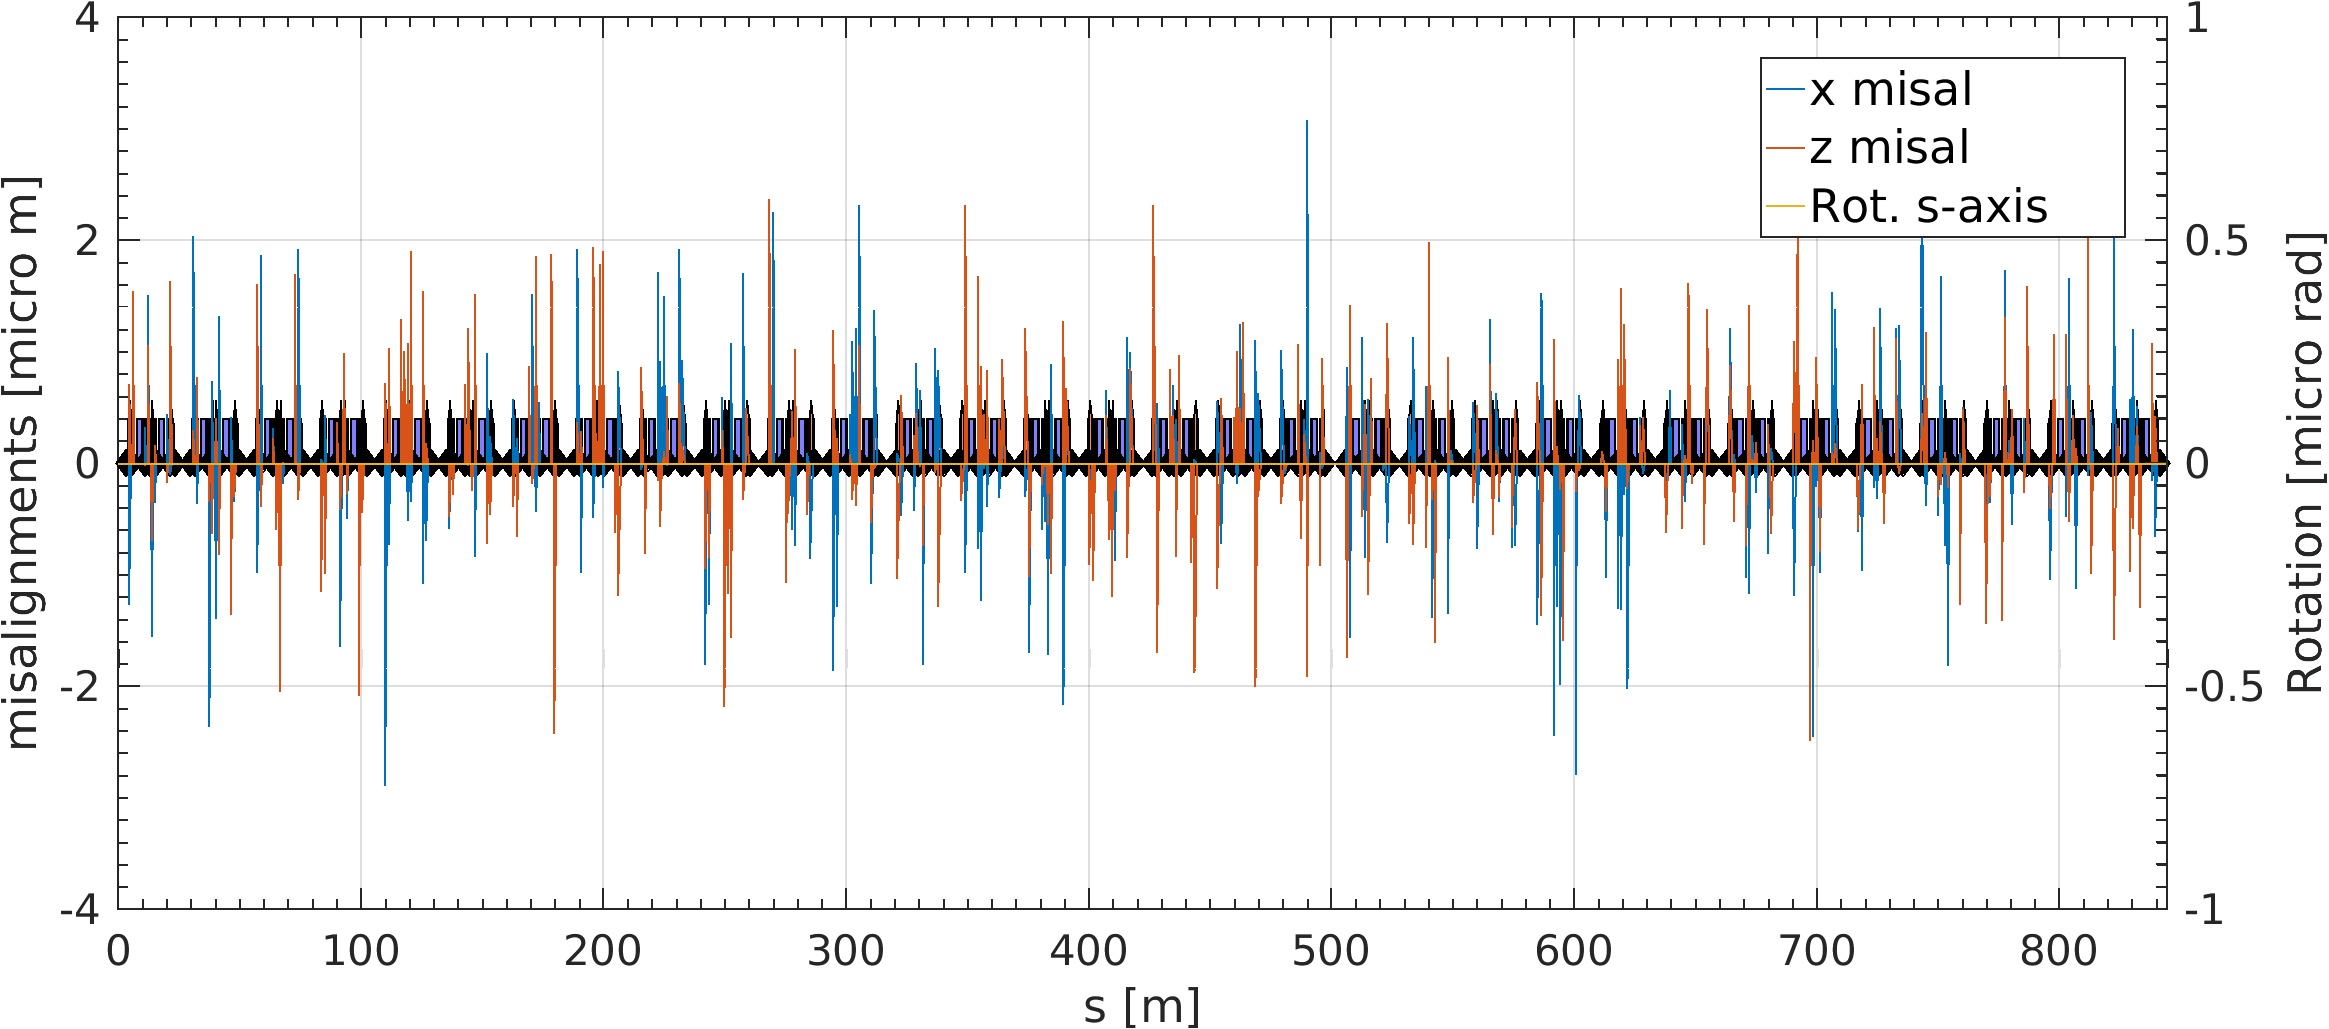
\includegraphics[width=0.7\textwidth]{C:/Users/liuzzo/Desktop/LatexDocuments/ATErrorAndCorrection/images/DxDy/SetErrDxDy.jpg}
	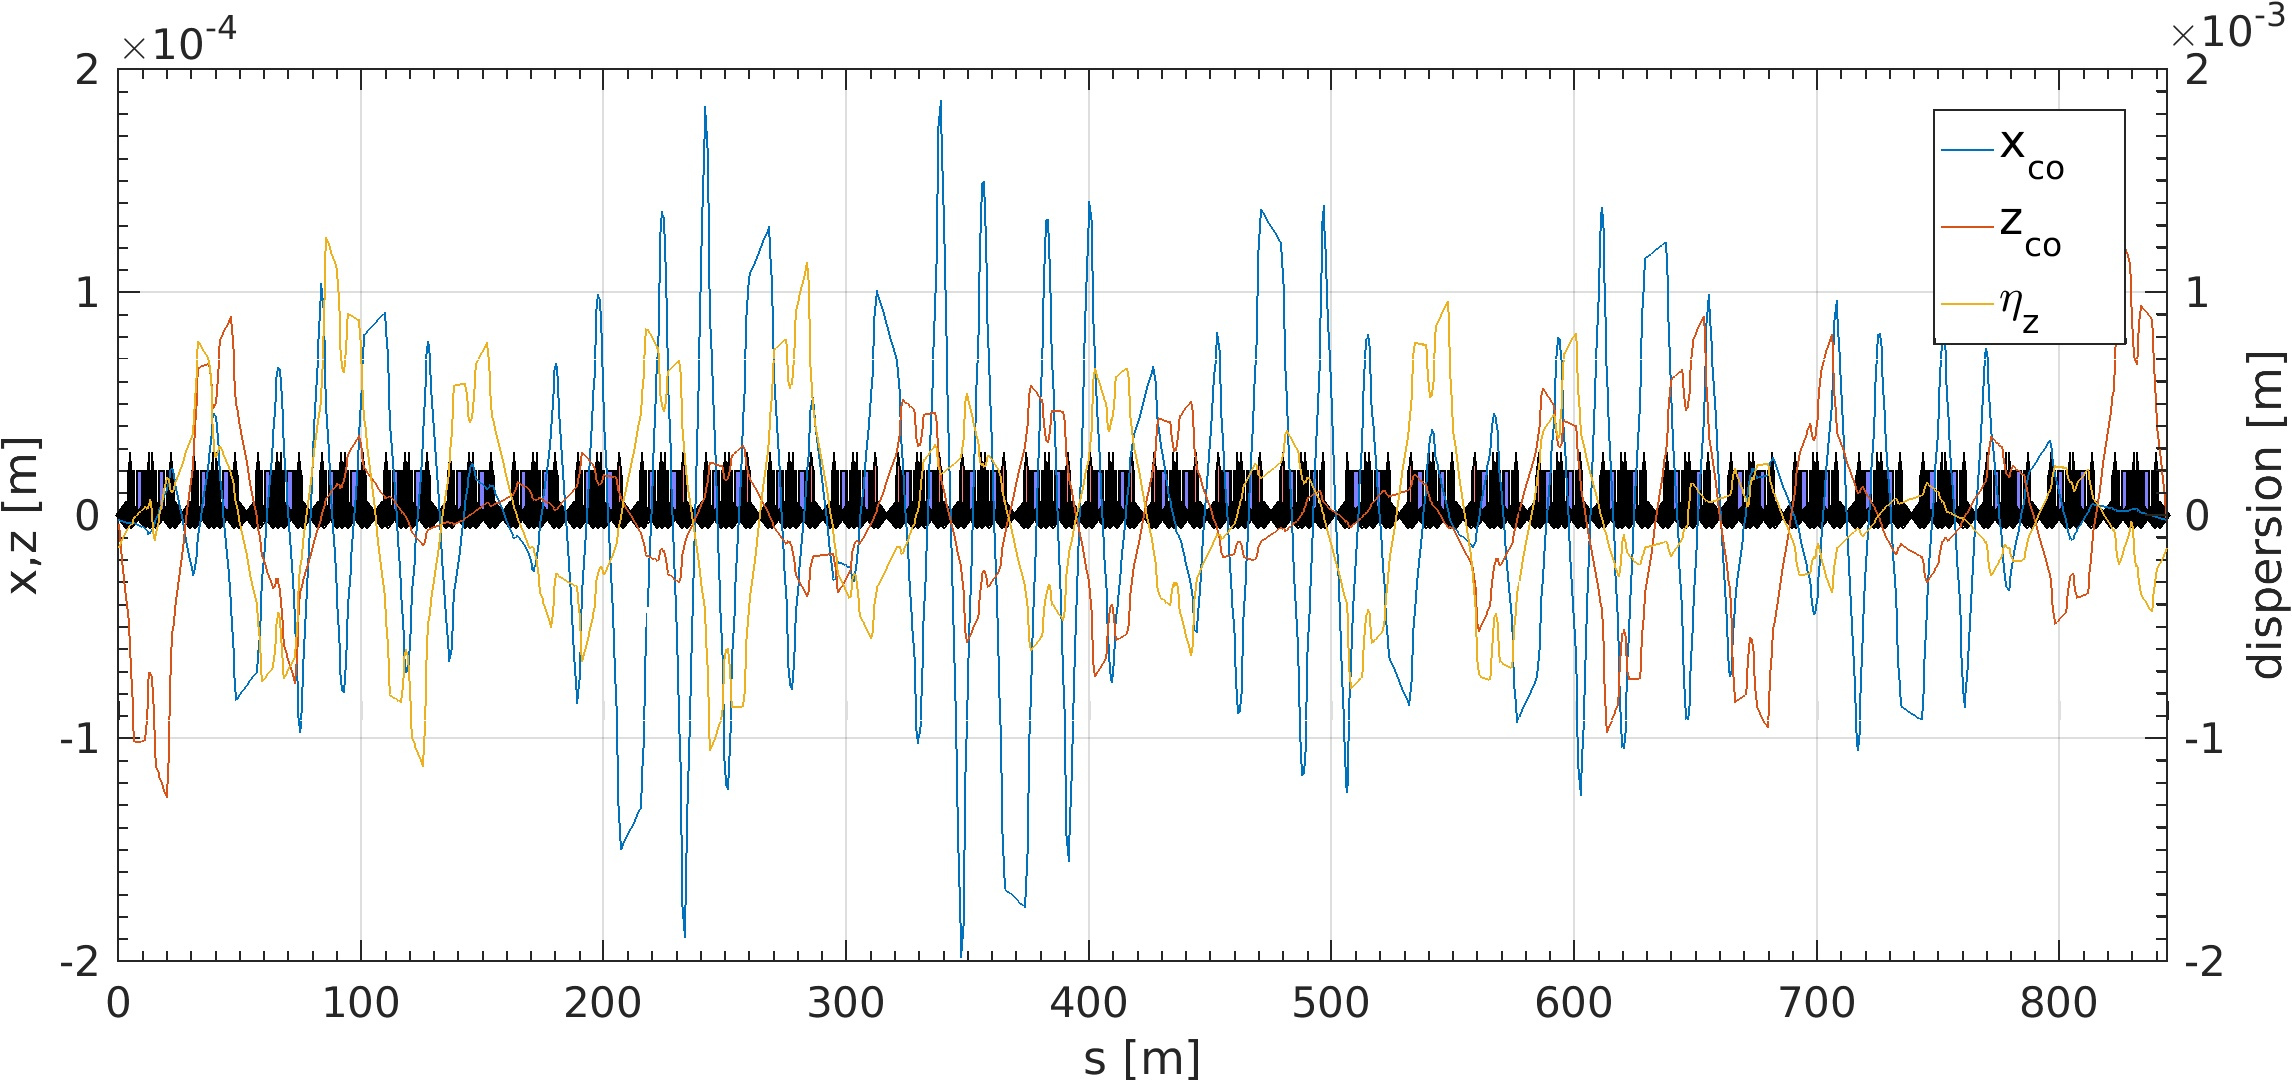
\includegraphics[width=0.7\textwidth]{C:/Users/liuzzo/Desktop/LatexDocuments/ATErrorAndCorrection/images/DxDy/OrbitWithErr.jpg}
	\caption{top: random errors from a Gaussian distribution with $\sigma=\SI{1}{\micro m}$,\\ bottom: closed orbit and vertical dispersion with errors}
	\label{fig:dxdy}
\end{figure}

\clearpage
\subsubsection*{Rotation about the s-axis}
Below an example of rotation of quadrupole magnets using the function \emph{atsettilt}. Figure \ref{fig:rot} presents the dispersion distortion obtained in this case.
 
\begin{lstlisting}
% get indexes
indq=find(atgetcells(ring,'Class','Quadrupole'));

% define s-axis rotation errors
dt=1e-6*randn(size(indq)); % random errors of 1um

% set errors
ringerr=atsettilt(ring,indq,dt);
\end{lstlisting}

\begin{figure}[!h]
	\centering
		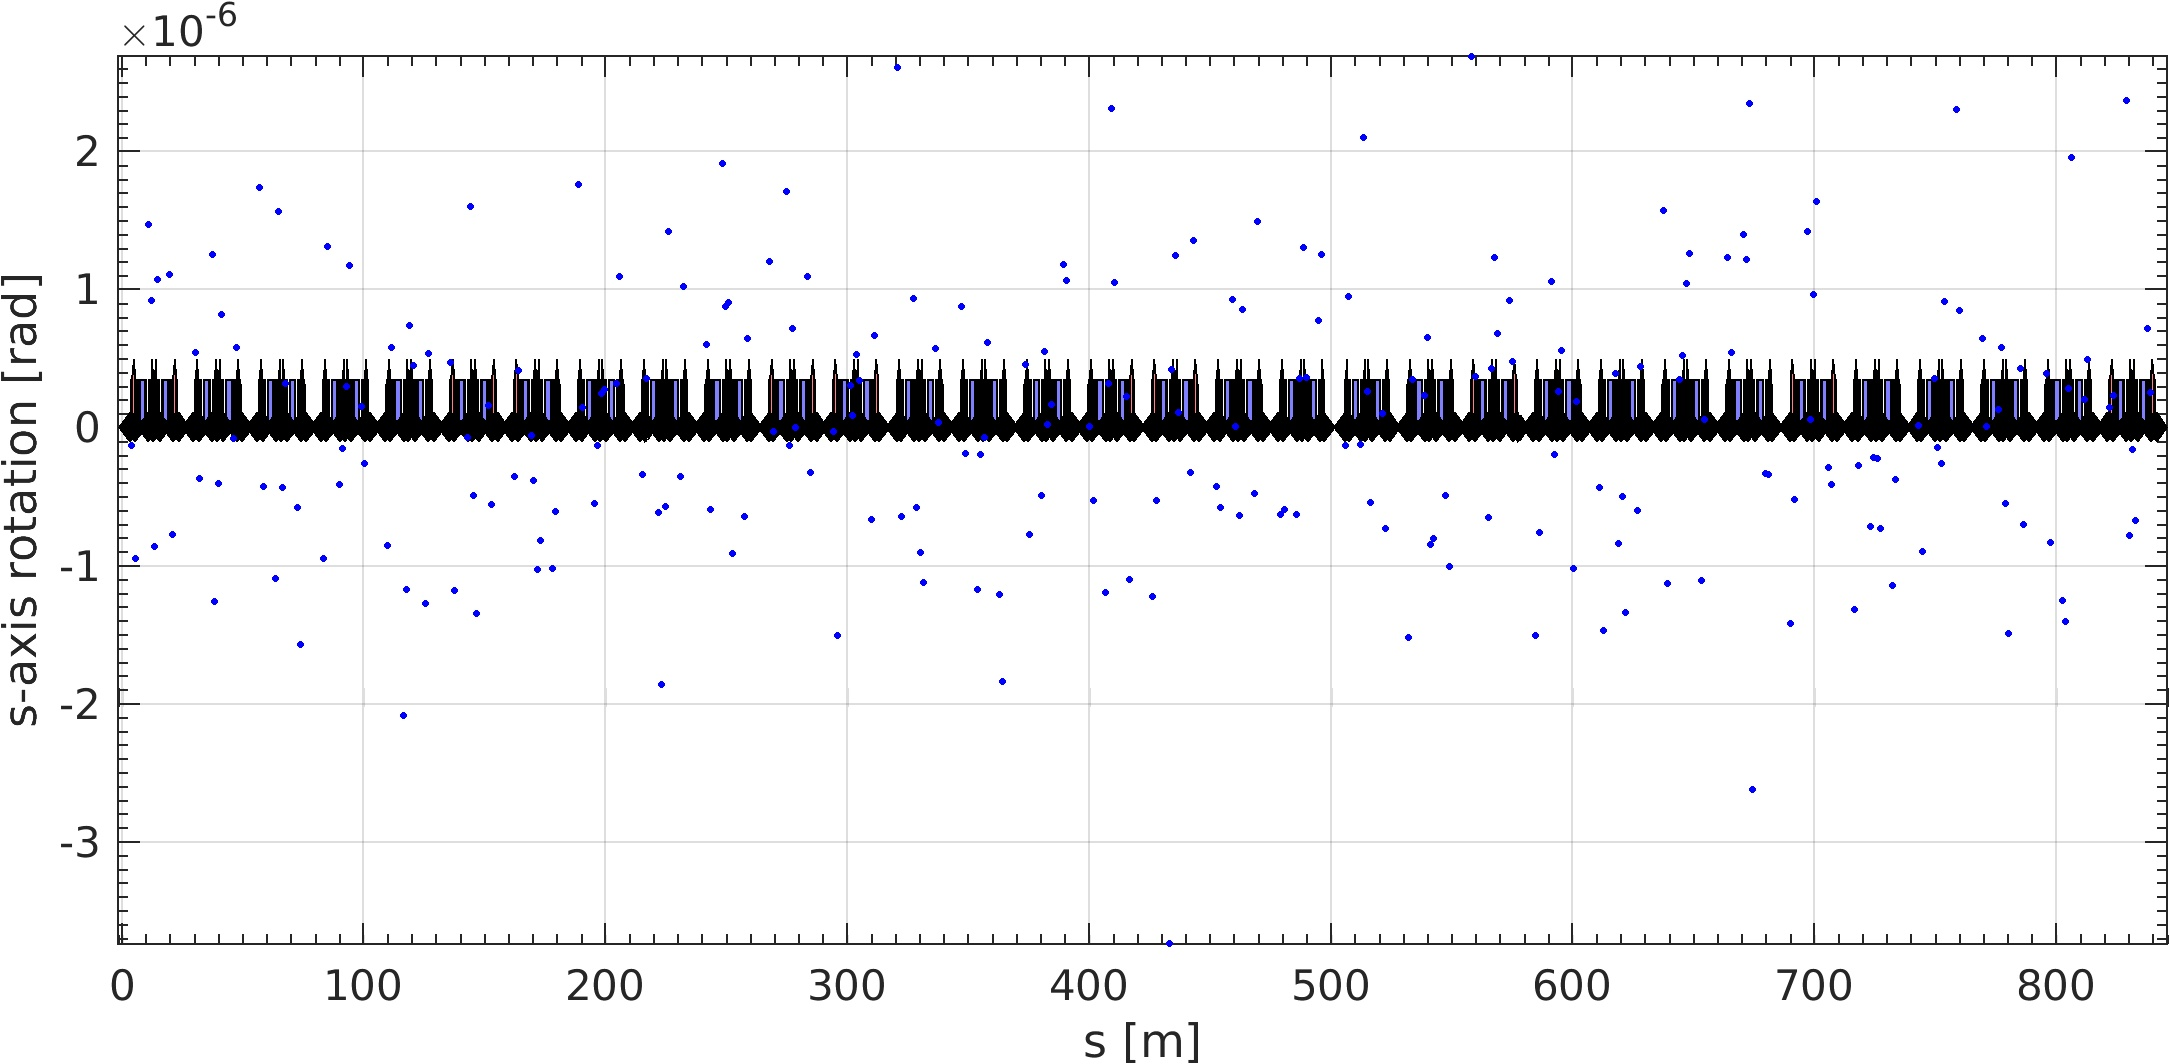
\includegraphics[width=0.98\textwidth]{./images/TILT/SetErrTilt.jpg}
	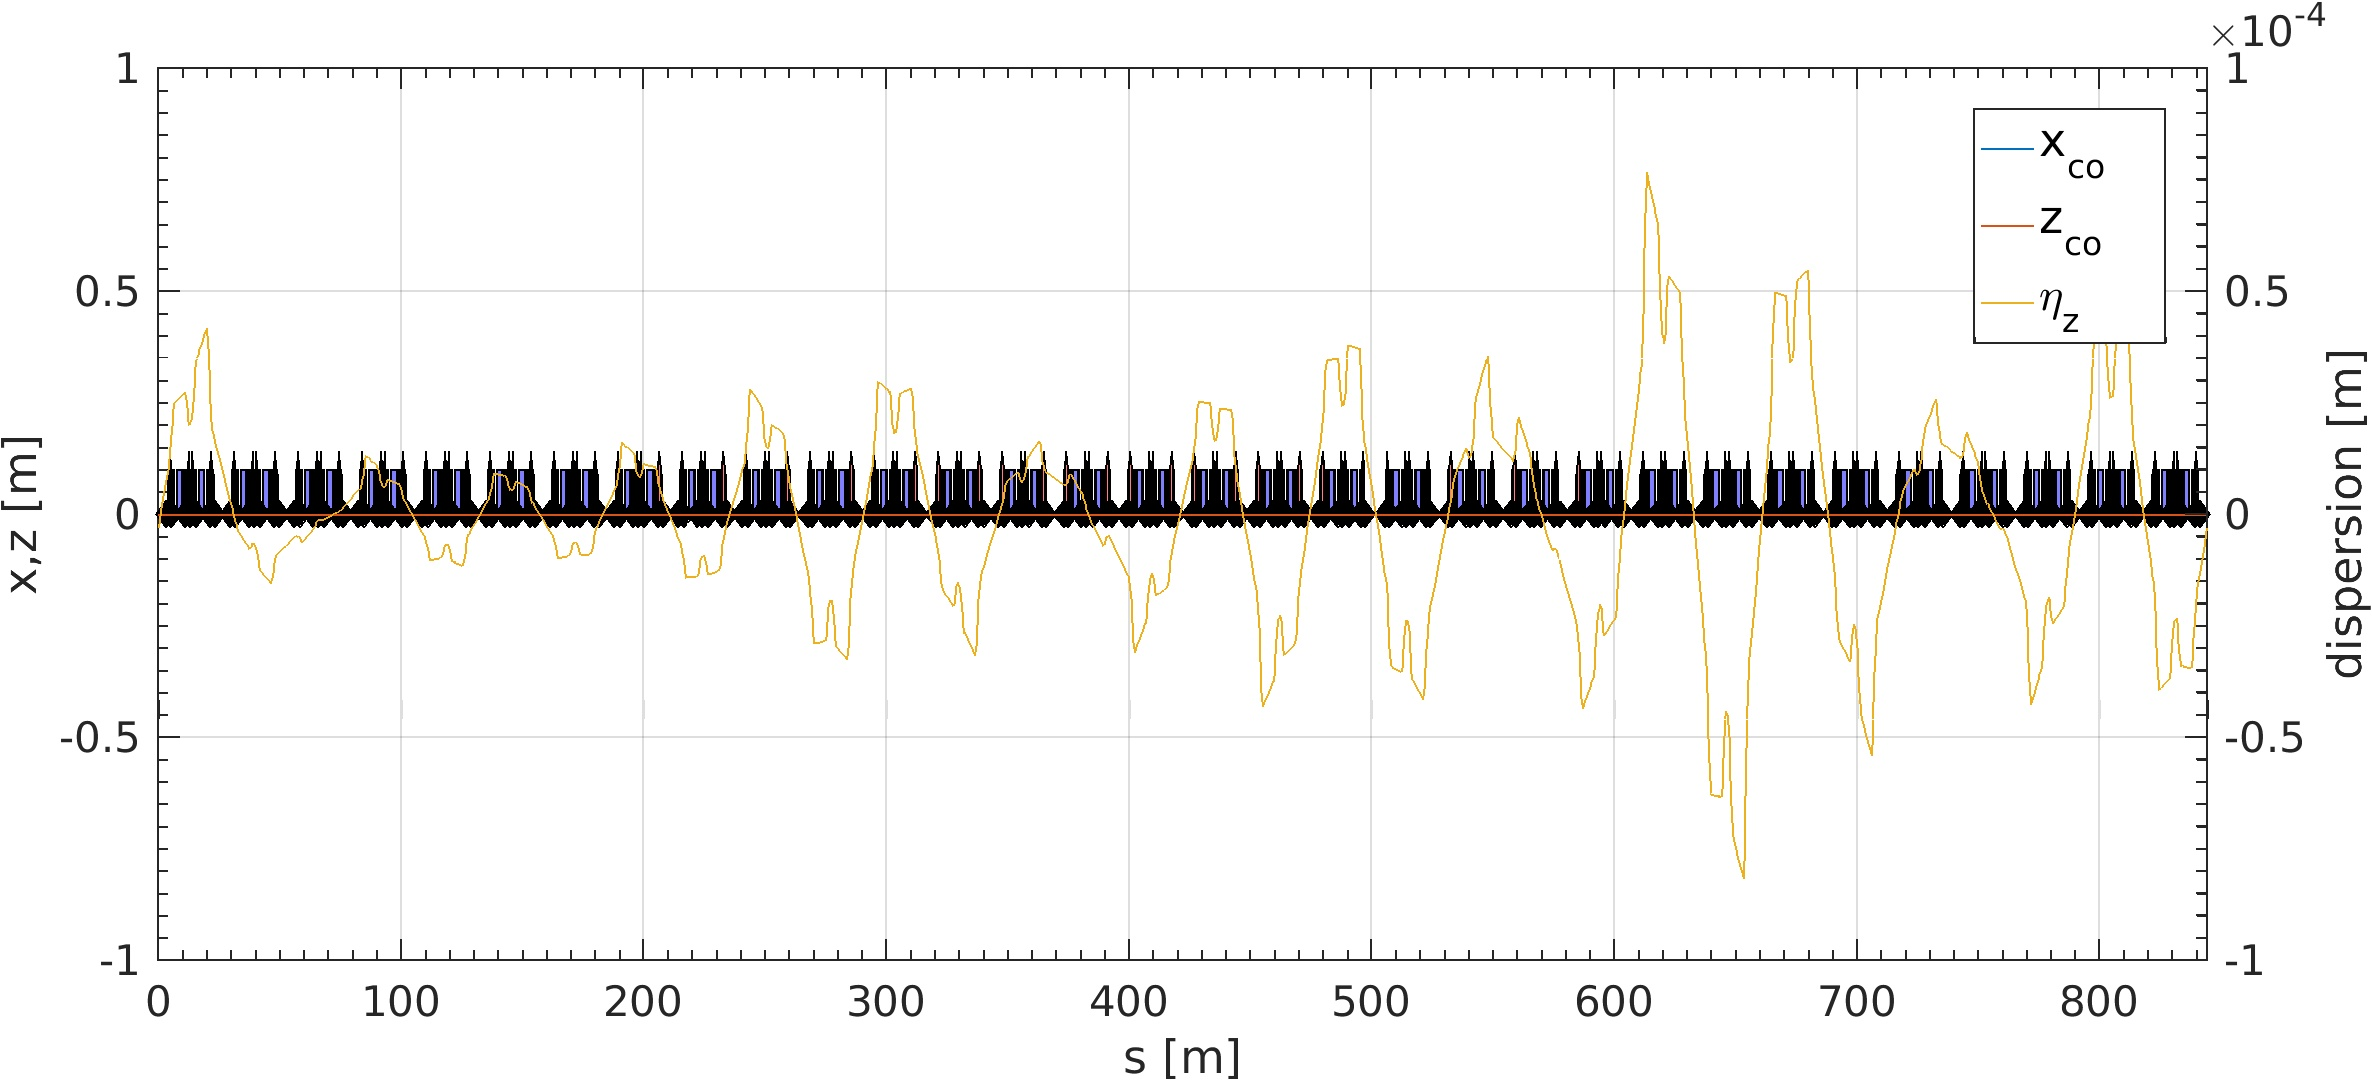
\includegraphics[width=0.98\textwidth]{./images/TILT/OrbitWithErrTilt.jpg}
	\caption{top: random s-axis rotation errors from a Gaussian distribution with $\sigma=\SI{1}{\micro rad}$,\\ bottom: closed orbit and vertical dispersion with s-axis rotation errors}
	\label{fig:rot}
\end{figure}

\clearpage
\subsubsection*{Rotation of a dipole about the s-axis}

Dipoles change the reference frame but their field is usually ignored.
To evidence the effect of dipole rotation and field errors those must be expressed in terms of \emph{PolynomA} and \emph{PolynomB}. The function \emph{atsettiltdipole} implements this feature, and sets the field PolynomB and PolynomA in a dipole to represent the distortion introduced by the rotated bending magnet. In the figures below the effect of the rotation of a dipole are shown in three cases: rotation of a straight multipole using \emph{atsettilt} (Fig.\ref{fig:multtilt}), rotation of a dipole using \emph{atsettilt} (Fig.\ref{fig:diptiltref}), rotation of a dipole using \ref{atsettiltdipole} (Fig.\ref{fig:diptilt}).

\begin{figure}[!thb]
	\centering
	\begin{subfigure}[b]{\textwidth}
        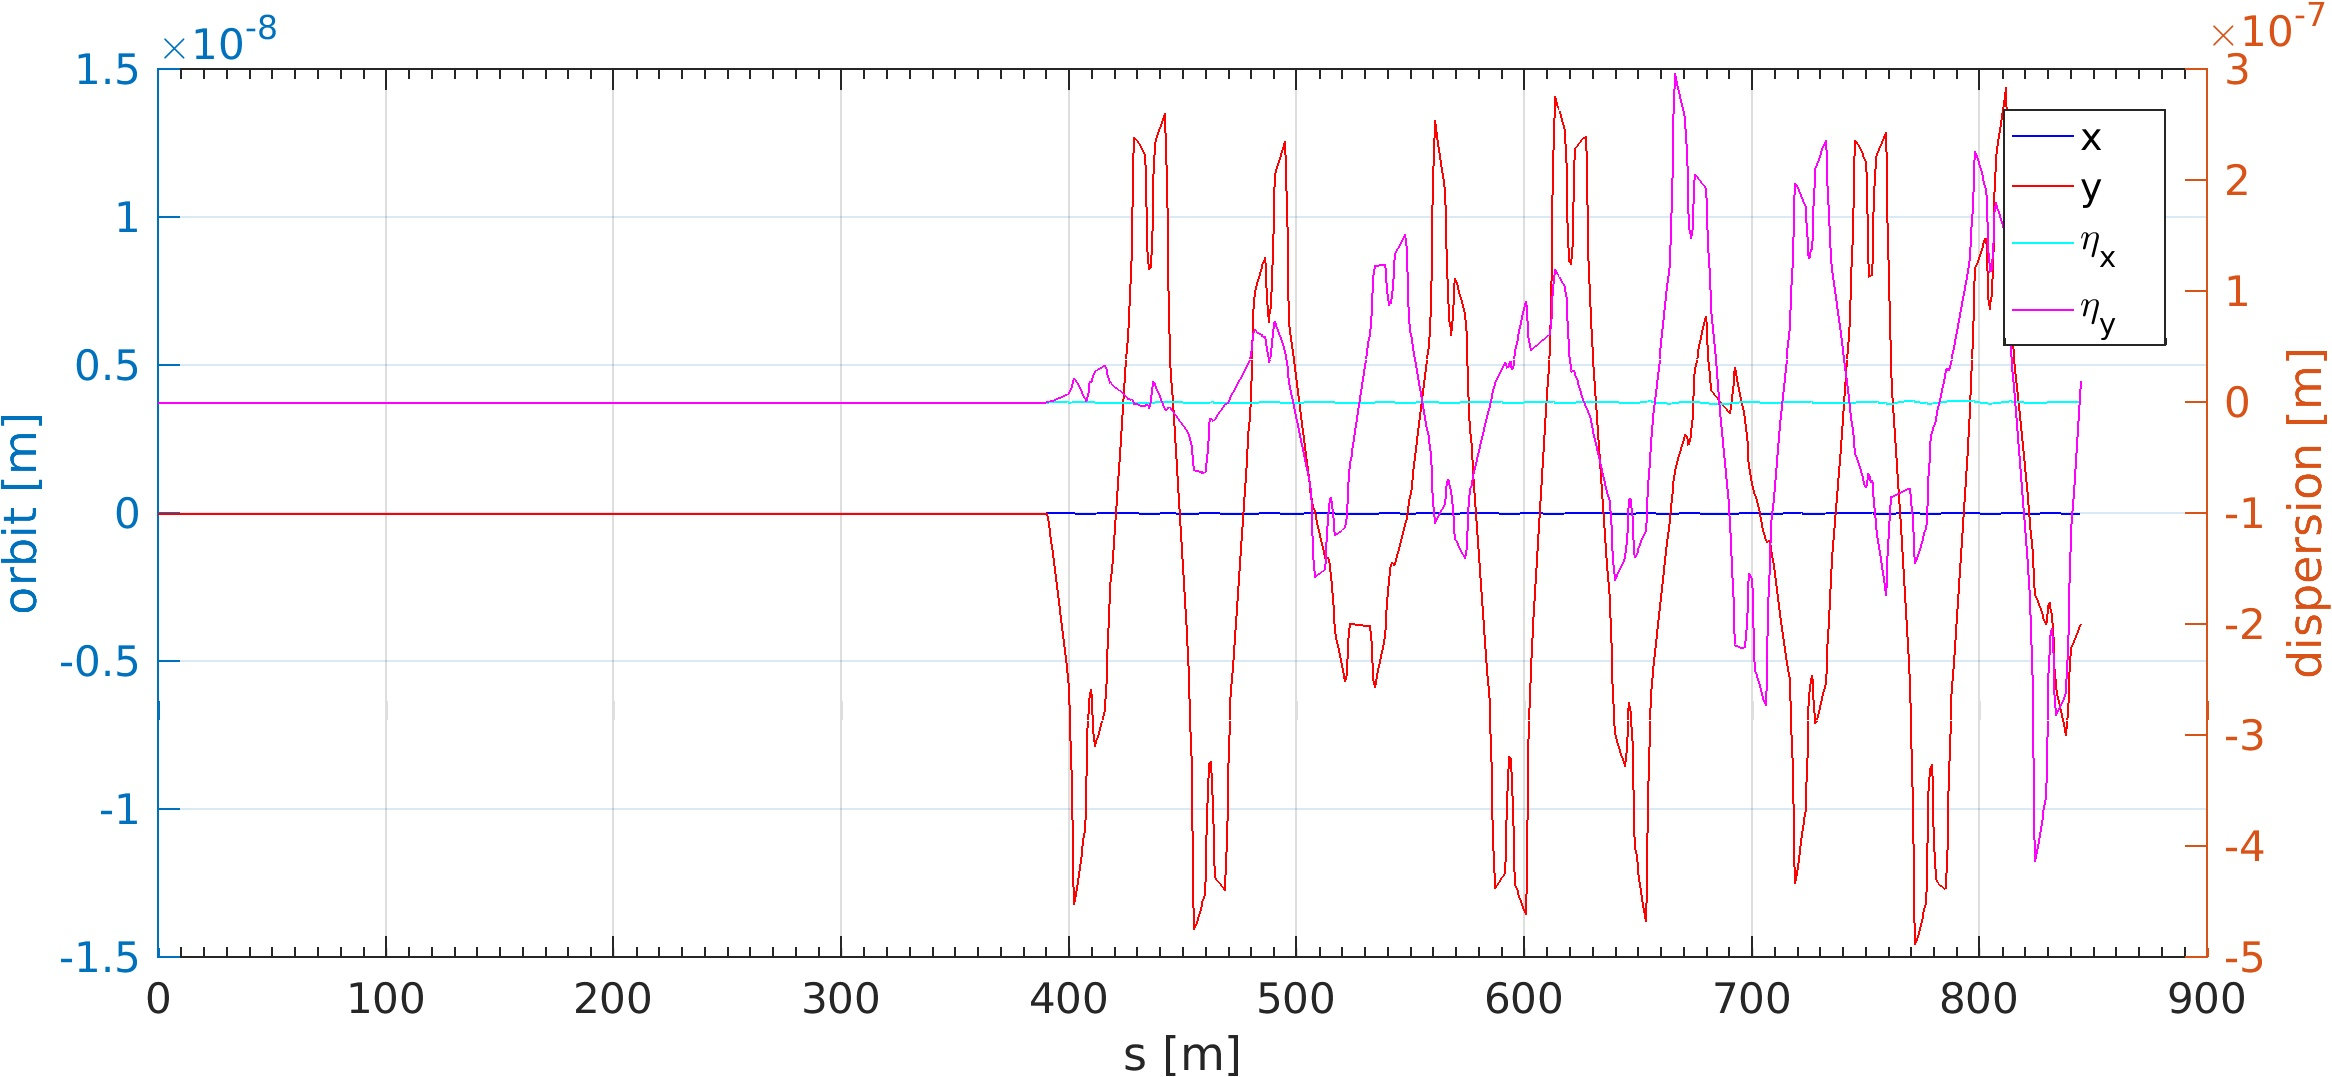
\includegraphics[width=0.98\textwidth]{./images/TILT/OrbitDispCorTiltVar.jpg}
	\caption{Multipole kick rotated using \emph{atsettilt}}
        \label{fig:multtilt}
    \end{subfigure}
		
	\begin{subfigure}[b]{\textwidth}
        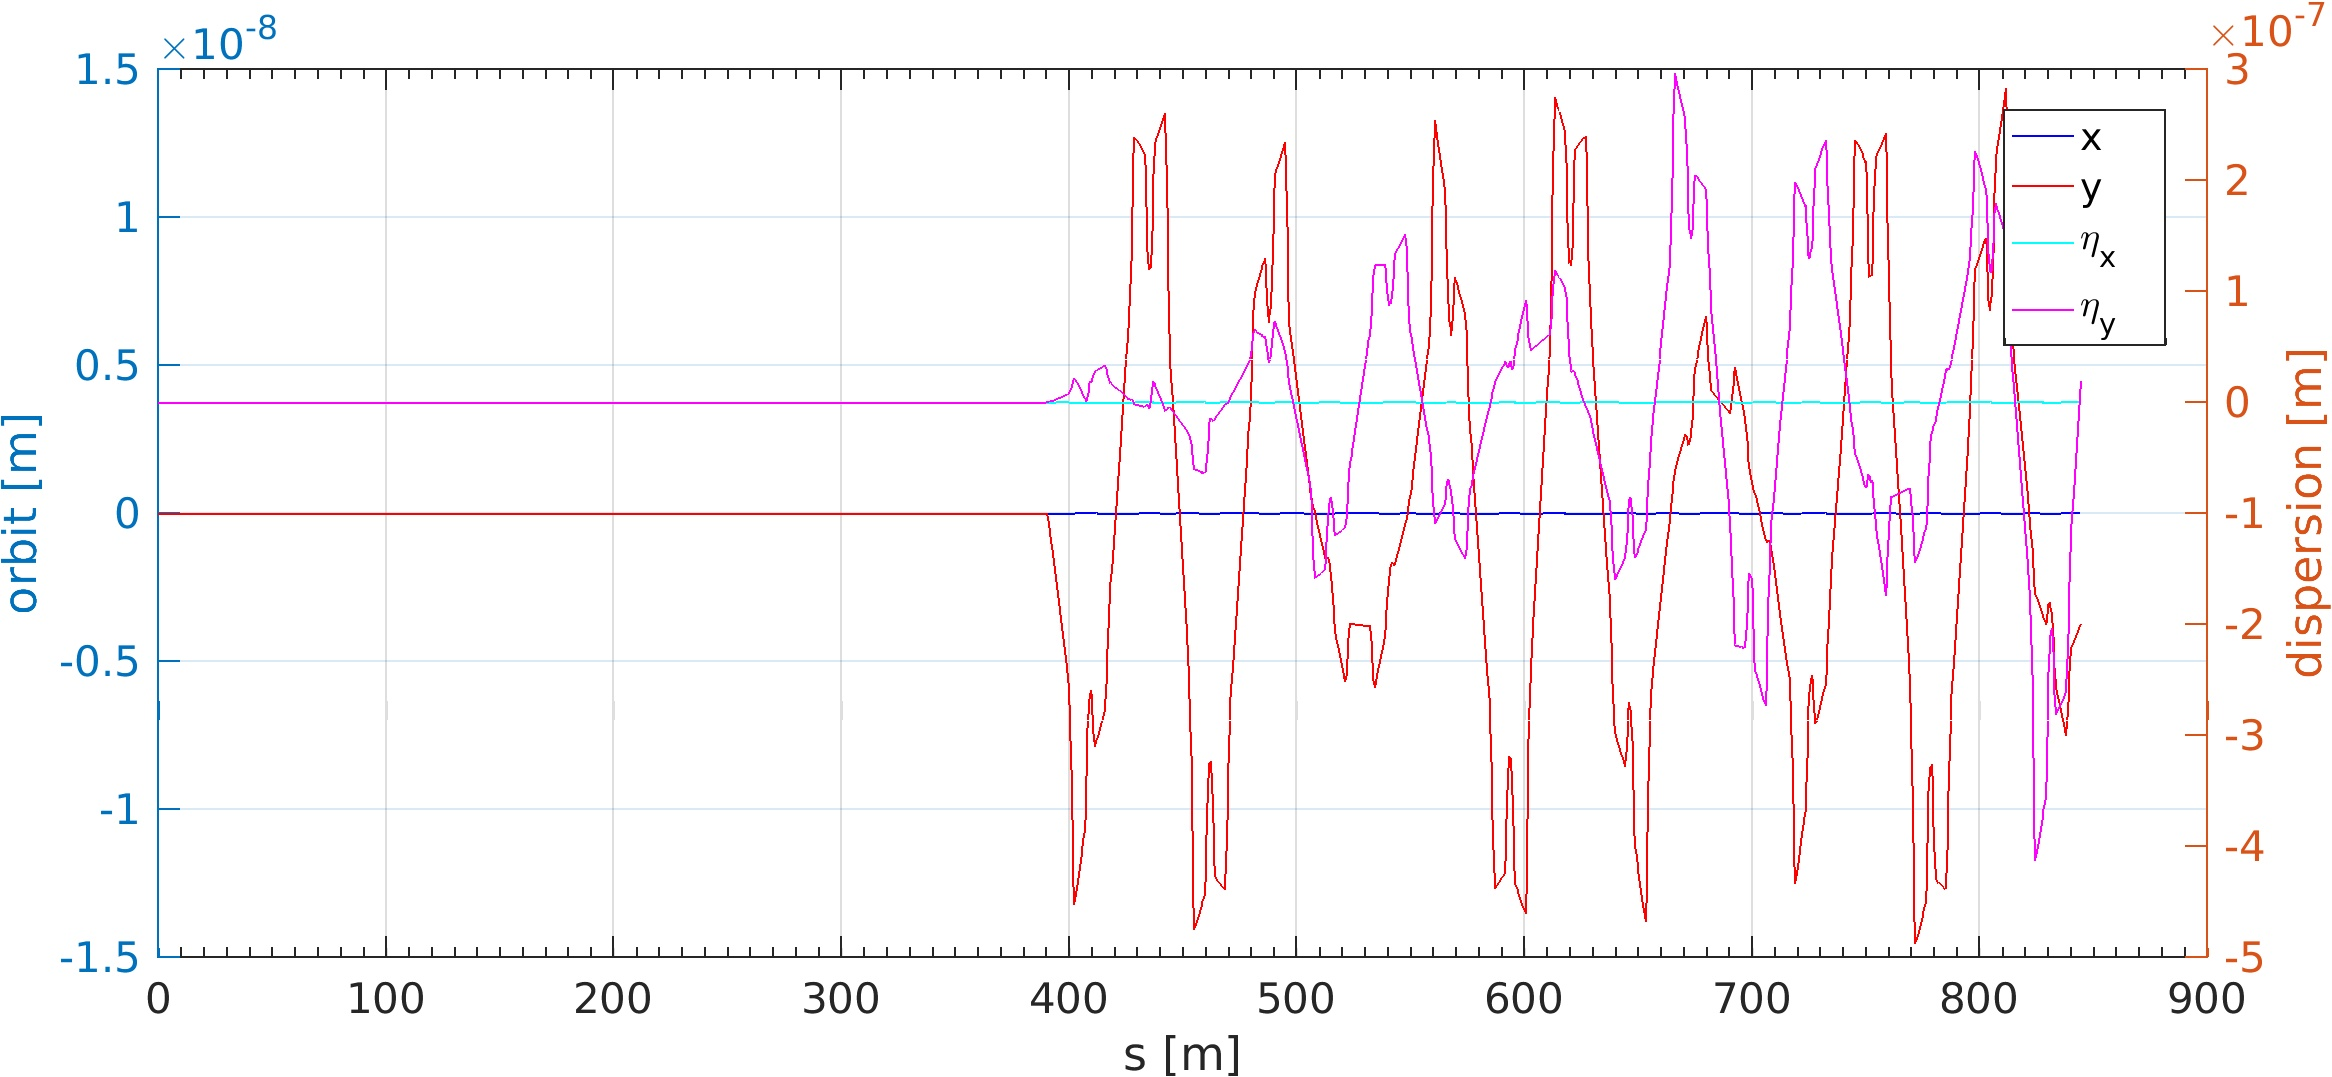
\includegraphics[width=0.98\textwidth]{./images/TILT/OrbitDispDipTiltVar.jpg}
	\caption{Dipole rotated using \emph{atsettiltdipole}}
        \label{fig:diptilt}
    \end{subfigure}
	
	\begin{subfigure}[b]{\textwidth}
        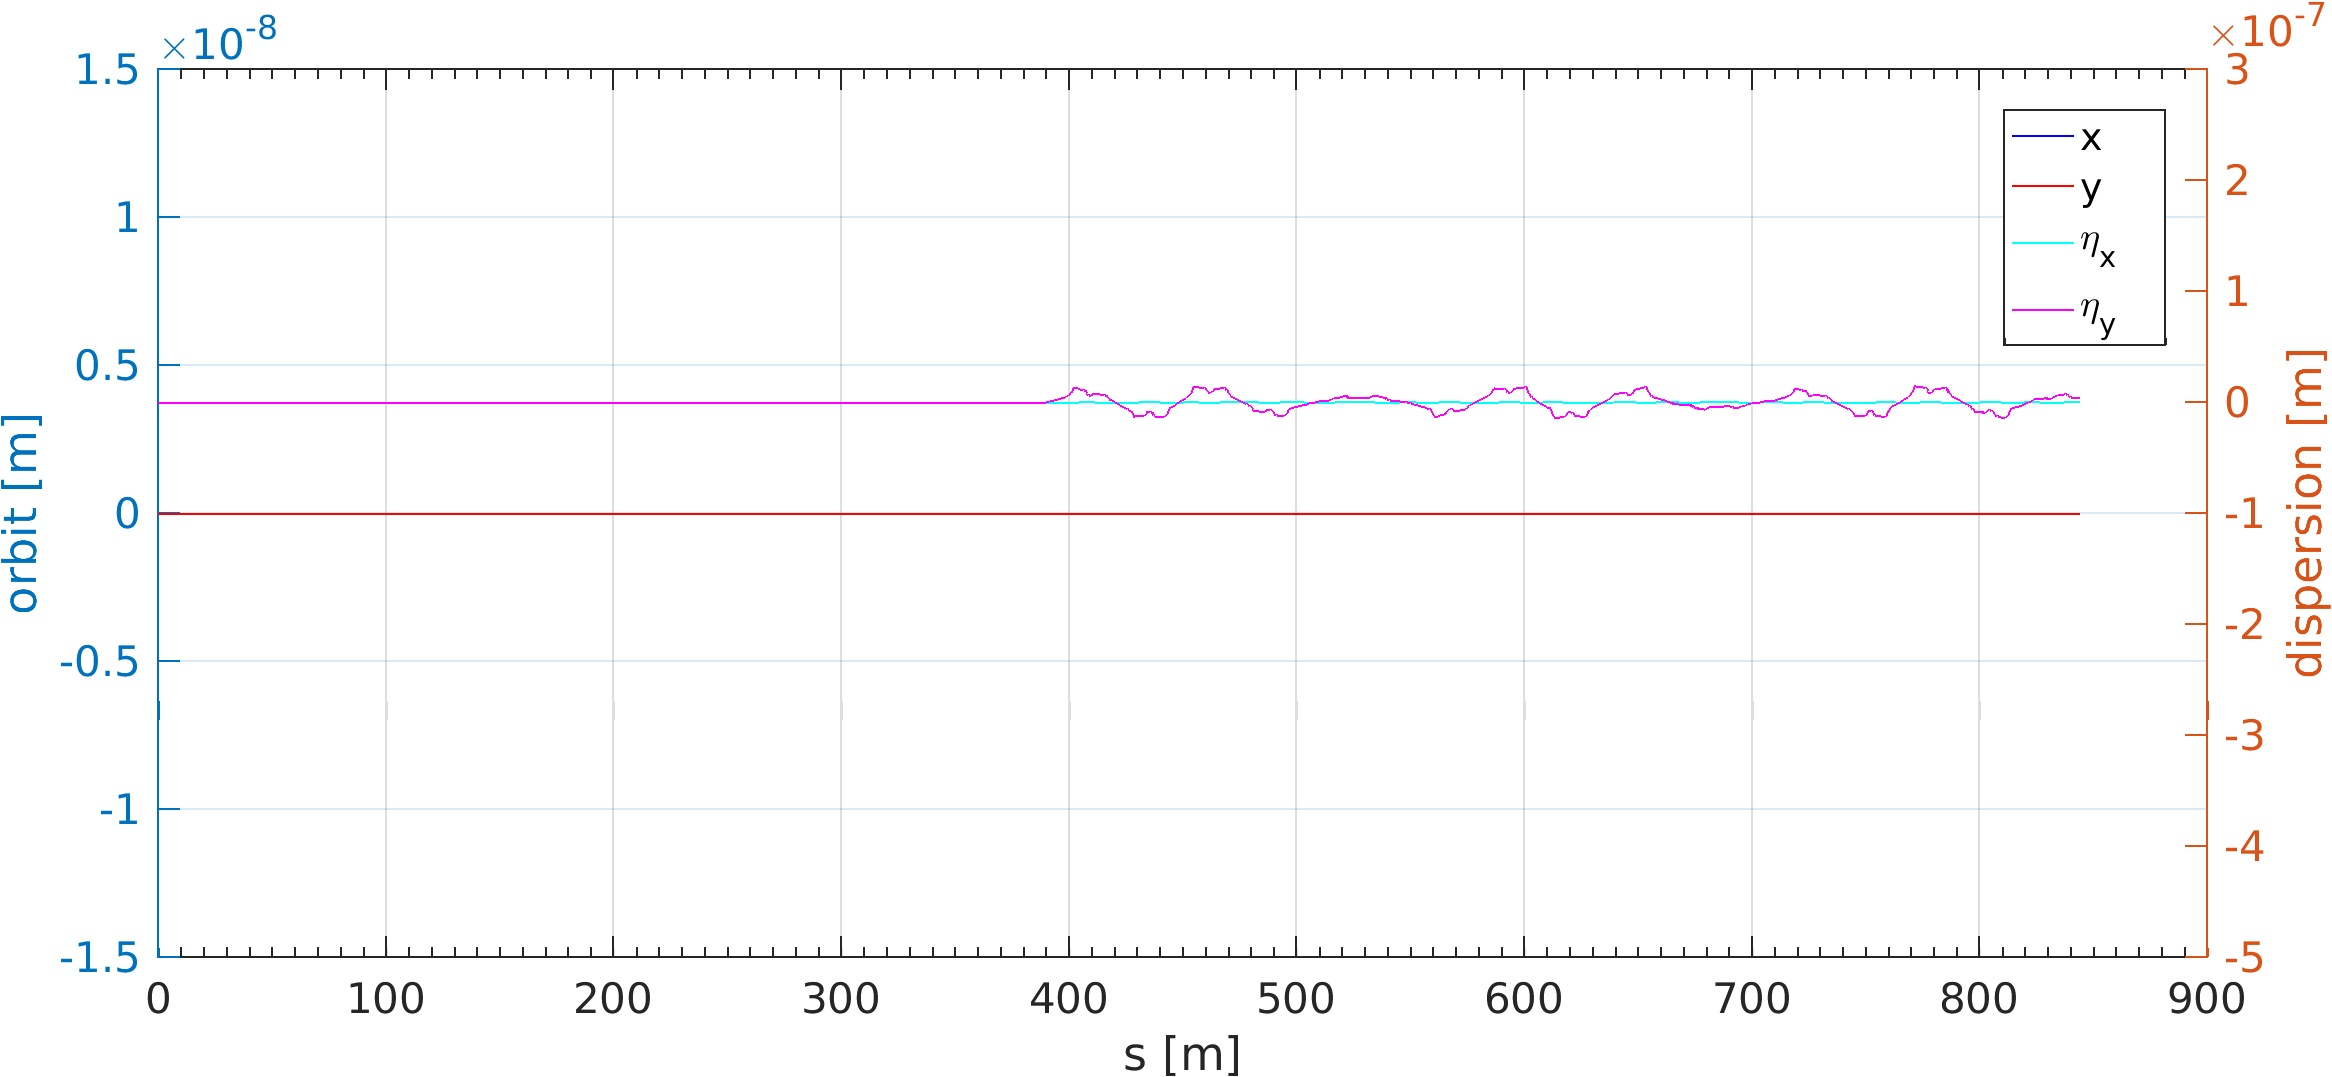
\includegraphics[width=0.98\textwidth]{./images/TILT/OrbitDispDipTiltVarRef.jpg}
	\caption{Dipole rotated using \emph{atsettilt}}
        \label{fig:diptiltref}
    \end{subfigure}
	\caption{Orbit and dispersion variation when tilting by $100\, \mu rad$ a $10 \mu rad$ horizontal kick at about $390\,m$.}
	\label{fig:rotdipvscor}
\end{figure}

There is no difference between \ref{fig:multtilt} and \ref{fig:diptilt}, while the tilt implemented rotating the reference system does not show the expected orbit distortion.

The same considerations are ture for the rotation of a combined function dipole-quadrupole in figure \ref{fig:dipquadrot}. 


\clearpage
\subsection*{Rotation about x and y axis}
These two rotation are implemented using the fields \emph{T1} and \emph{T2}. 



\clearpage
\subsubsection*{Longitudinal alignment errors}
Longitudinal alignment errors require to change the length of adjacent drift spaces. For Dipoles also a change of trajectory needs to be considered (see Fig. \ref{fig:dipdsscheme}). the length of the lattice changes when displacing longitudinally dipoles.

\begin{lstlisting}
% get indexes
inddip=find(atgetcells(ring,'Class','Dipole'));

% define longitudinal displacement
DS=-1e-2; 

% set fixed -1cm displacement at first 2 dipoles in the lattice
ringerr=atset_s_shift(ring,inddip([1,2]),DS);

\end{lstlisting}

\begin{figure}[!thb]
	\centering
	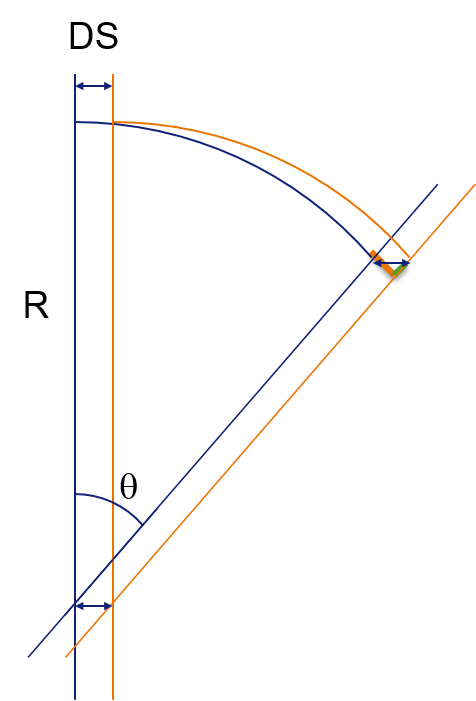
\includegraphics[width=0.38\textwidth]{./images/LongitudinalDisplacement/DipoleDS.png}
	\caption{Longitudinal displacements of dipole.}
	\label{fig:dipdsscheme}
\end{figure}

\begin{figure}[!thb]
	\centering
	\begin{subfigure}[b]{\textwidth}
        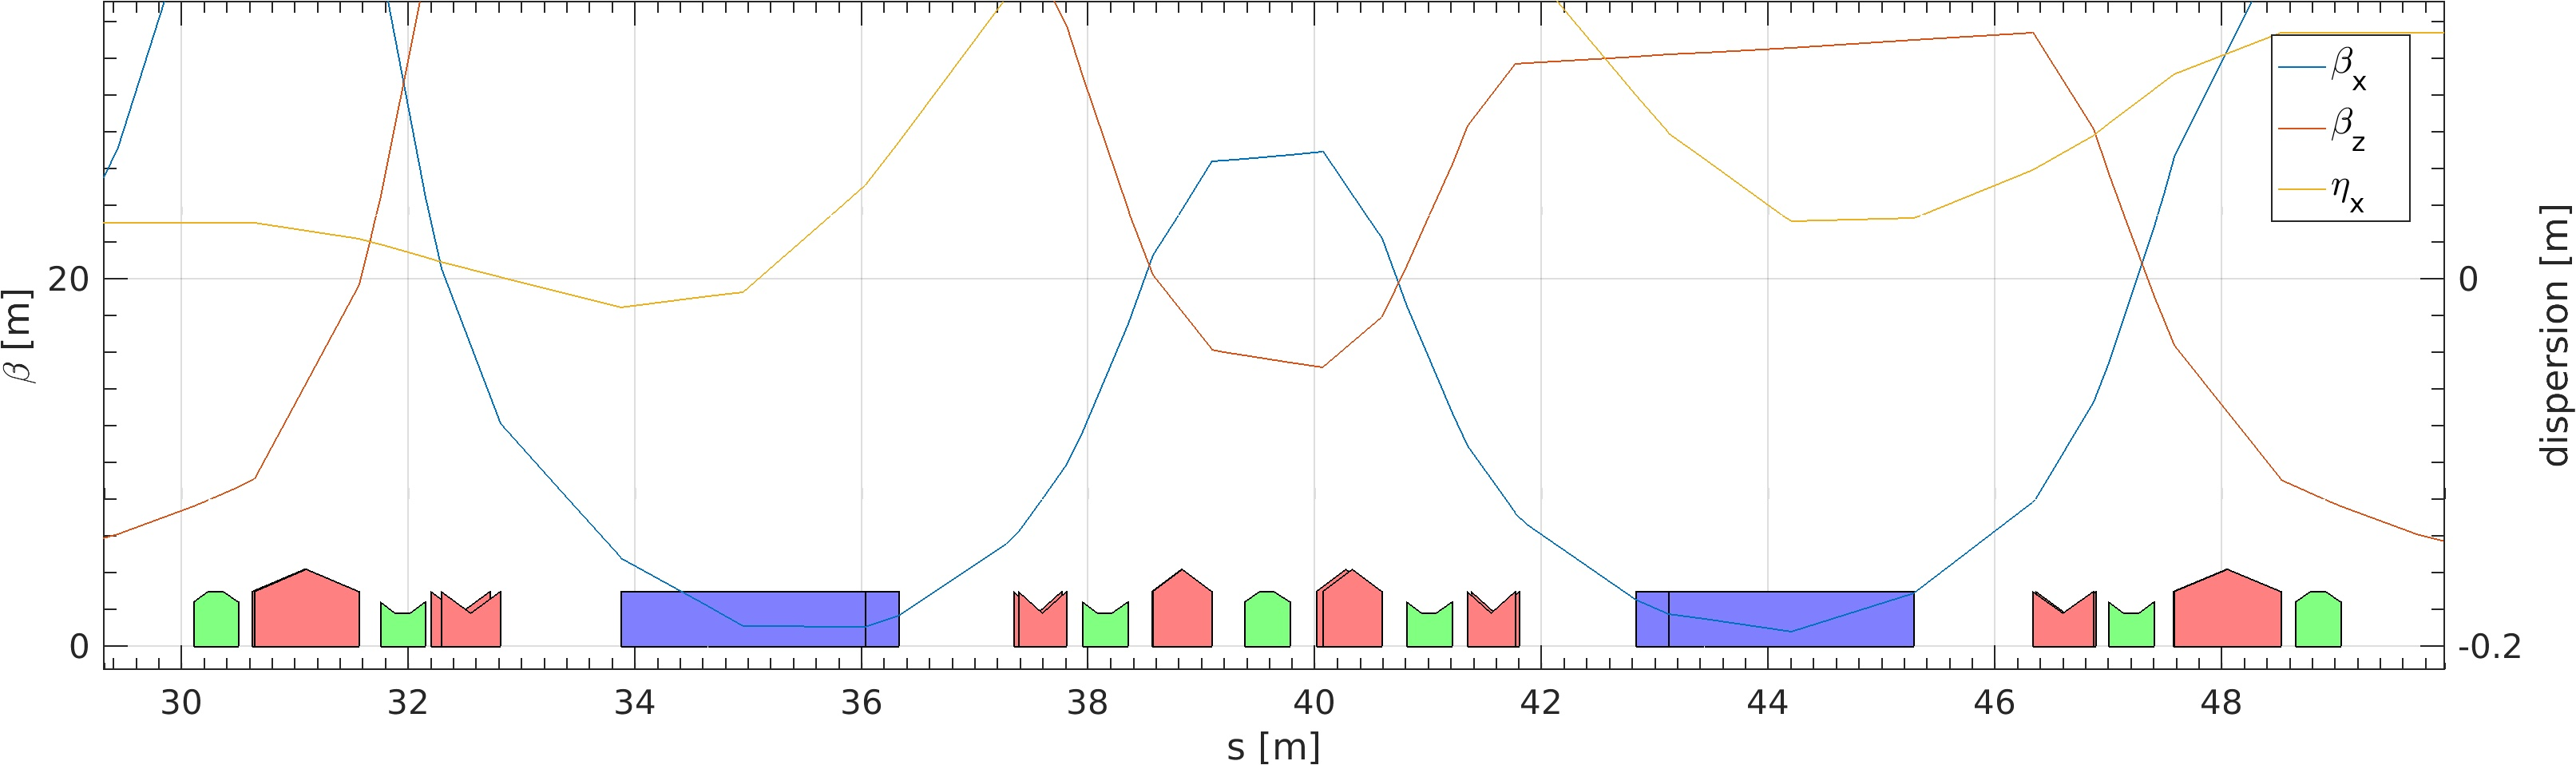
\includegraphics[width=0.98\textwidth]{./images/LongitudinalDisplacement/DeltaSQuadZoom.jpg}
	\caption{Quadrupoles longitudinally displaced}
        \label{fig:quadsDs}
    \end{subfigure}
		
	\begin{subfigure}[b]{\textwidth}
        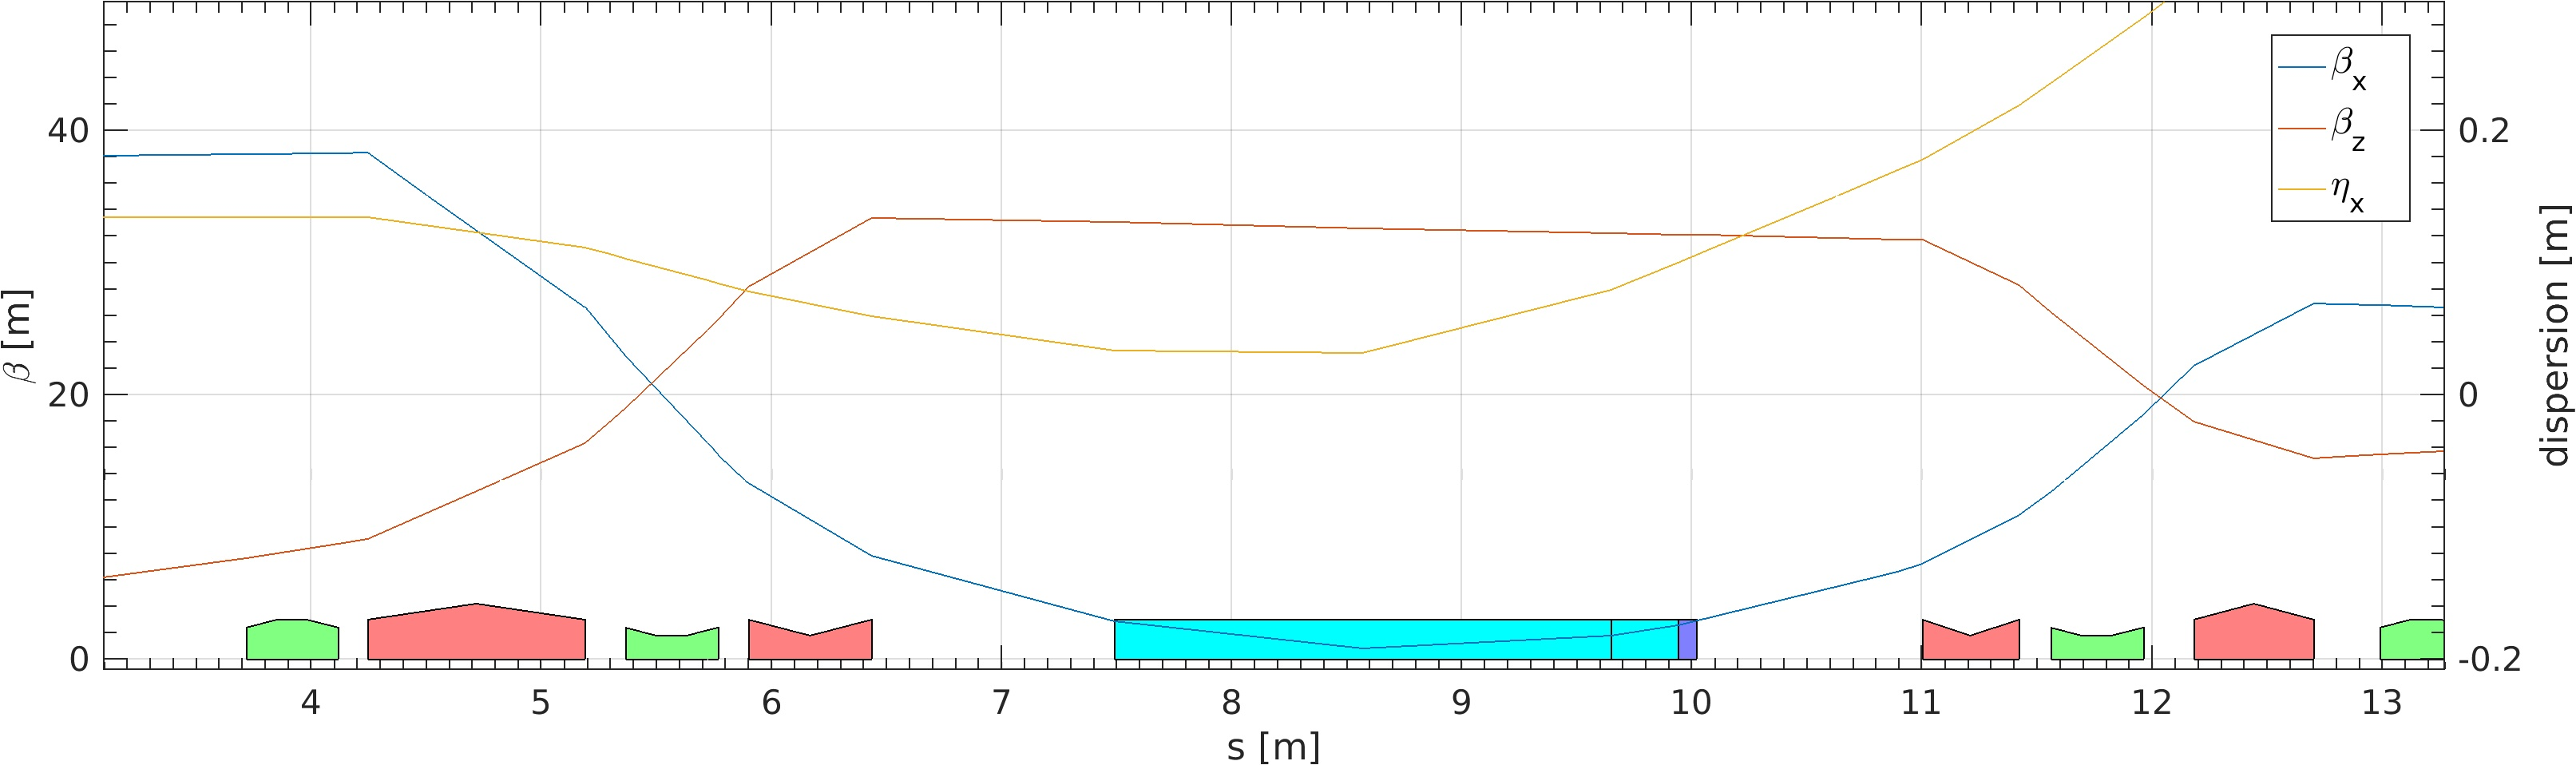
\includegraphics[width=0.98\textwidth]{./images/LongitudinalDisplacement/DeltaSDipZoom.jpg}
	\caption{Dipole longitudinally displaced.}
        \label{fig:dipds}
    \end{subfigure}
	\caption{Longitudinal displacements.}
	\label{fig:dipquadrot}
\end{figure}


\subsection*{functions mentioned in the above section}
\begin{itemize}
	\item atsetshift
	\item atsettilt
	\item atsettiltdipole 
	\item atset_s_shift
\end{itemize}

\clearpage
\subsection{BPM errors}
BPM errors are: offset, rotation, gain and reading precision (random). Those are set in the lattice with the function \emph{atsetbpmerr}. 
\begin{lstlisting}
% get indexes
indm=find(atgetcells(ring,'Class','Monitor'));

% define bpm offset and rotation errors
ox=1e-5*randn(size(indm)); % random offset errors of 10um
oy=1e-5*randn(size(indm)); 
gx=1e-3*randn(size(indm)); % random gain errors of 0.1%
gy=1e-3*randn(size(indm));  
rx=1e-6; % reading error sigma of 1um (can also be a vector)
ry=1e-6;

% set errors in the lattice
ringerr=atsetbpmerr(ringerr,indm,ox,oy,gx,gy,rx,ry,rot);

\end{lstlisting}
To obtain BPM readings including the errors the function \emph{findorbit4Err} and \emph{findorbit6Err} are used. Below the simple function \emph{findorbit6Err} where the bpm errors are recovered and set on the orbit obtained by \emph{findorbit6Err}.
Future AT versions will try to implement this in a dedicated PassMethod in C, to increase the speed of this transformation. 

\begin{lstlisting}
function orbit = findorbit6Err(RING, indbpm,varargin)
% findorbit6 with bpm reading errors
%
%see also findorbit6 bpm_process bpm_matrices

orbit = findorbit6(RING, indbpm, varargin{:});

% read errors stored in BPM elements
useind=1:length(indbpm);
[rel,tel,trand] = bpm_matrices(RING(indbpm(useind)));

% modify x and y coordinate to consider the errors
bpmreading = bpm_process(orbit([1,3],:),rel,tel,trand);
orbit(1,:)=bpmreading(1,:);
orbit(3,:)=bpmreading(2,:);

\end{lstlisting}

Below a complete script to display the effect of BPM errors. 
\begin{lstlisting}
% get indexes
indm=find(atgetcells(ring,'Class','Monitor'));
indq=find(atgetcells(ring,'Class','Quadrupole'));
%ring=atsetfieldvalues(ring,indm,'PassMethod','MonitorPass');

% define quadrupole alignment and rotation errors
dx=1e-6*randn(size(indq)); % random errors of 1um
dy=1e-6*randn(size(indq)); % random errors of 1um
dt=1e-6*randn(size(indq)); % random errors of 1urad

% define bpm offset and rotation errors
ox=1e-5*randn(size(indm)); % random offset errors of 10um
oy=1e-5*randn(size(indm)); 
gx=1e-3*randn(size(indm)); % random gain errors of 0.1%
gy=1e-3*randn(size(indm));  
rx=1e-6; % reading error sigma of 1um (can also be a vector)
ry=1e-6; 
rot=1e-5*randn(size(indm)); % random rotation errors of 10urad

% set errors
ringerr=ring;
ringerr=atsetshift(ringerr,indq,dx,dy);
ringerr=atsettilt(ringerr,indq,dt);
ringerr=atsetbpmerr(ringerr,indm,ox,oy,gx,gy,rx,ry,rot);

% plots
figure('units','normalized','position',[0.1 0.4 0.65 0.35]);
s=findspos(ringerr,indm);
% no bpm errors
o=findorbit4(ringerr,0,indm);
plot(s,o(1,:)'*1e6,'k'); hold on;
% with bpm errors
oe=findorbit4Err(ringerr,0,indm);
plot(s,oe(1,:)'*1e6,'rx');

legend('orbit','bpm reading');
xlabel('s [m]');ylabel('x [\mum]')

\end{lstlisting}


\begin{figure}[!h]
	\centering
	\begin{subfigure}[b]{\textwidth}
  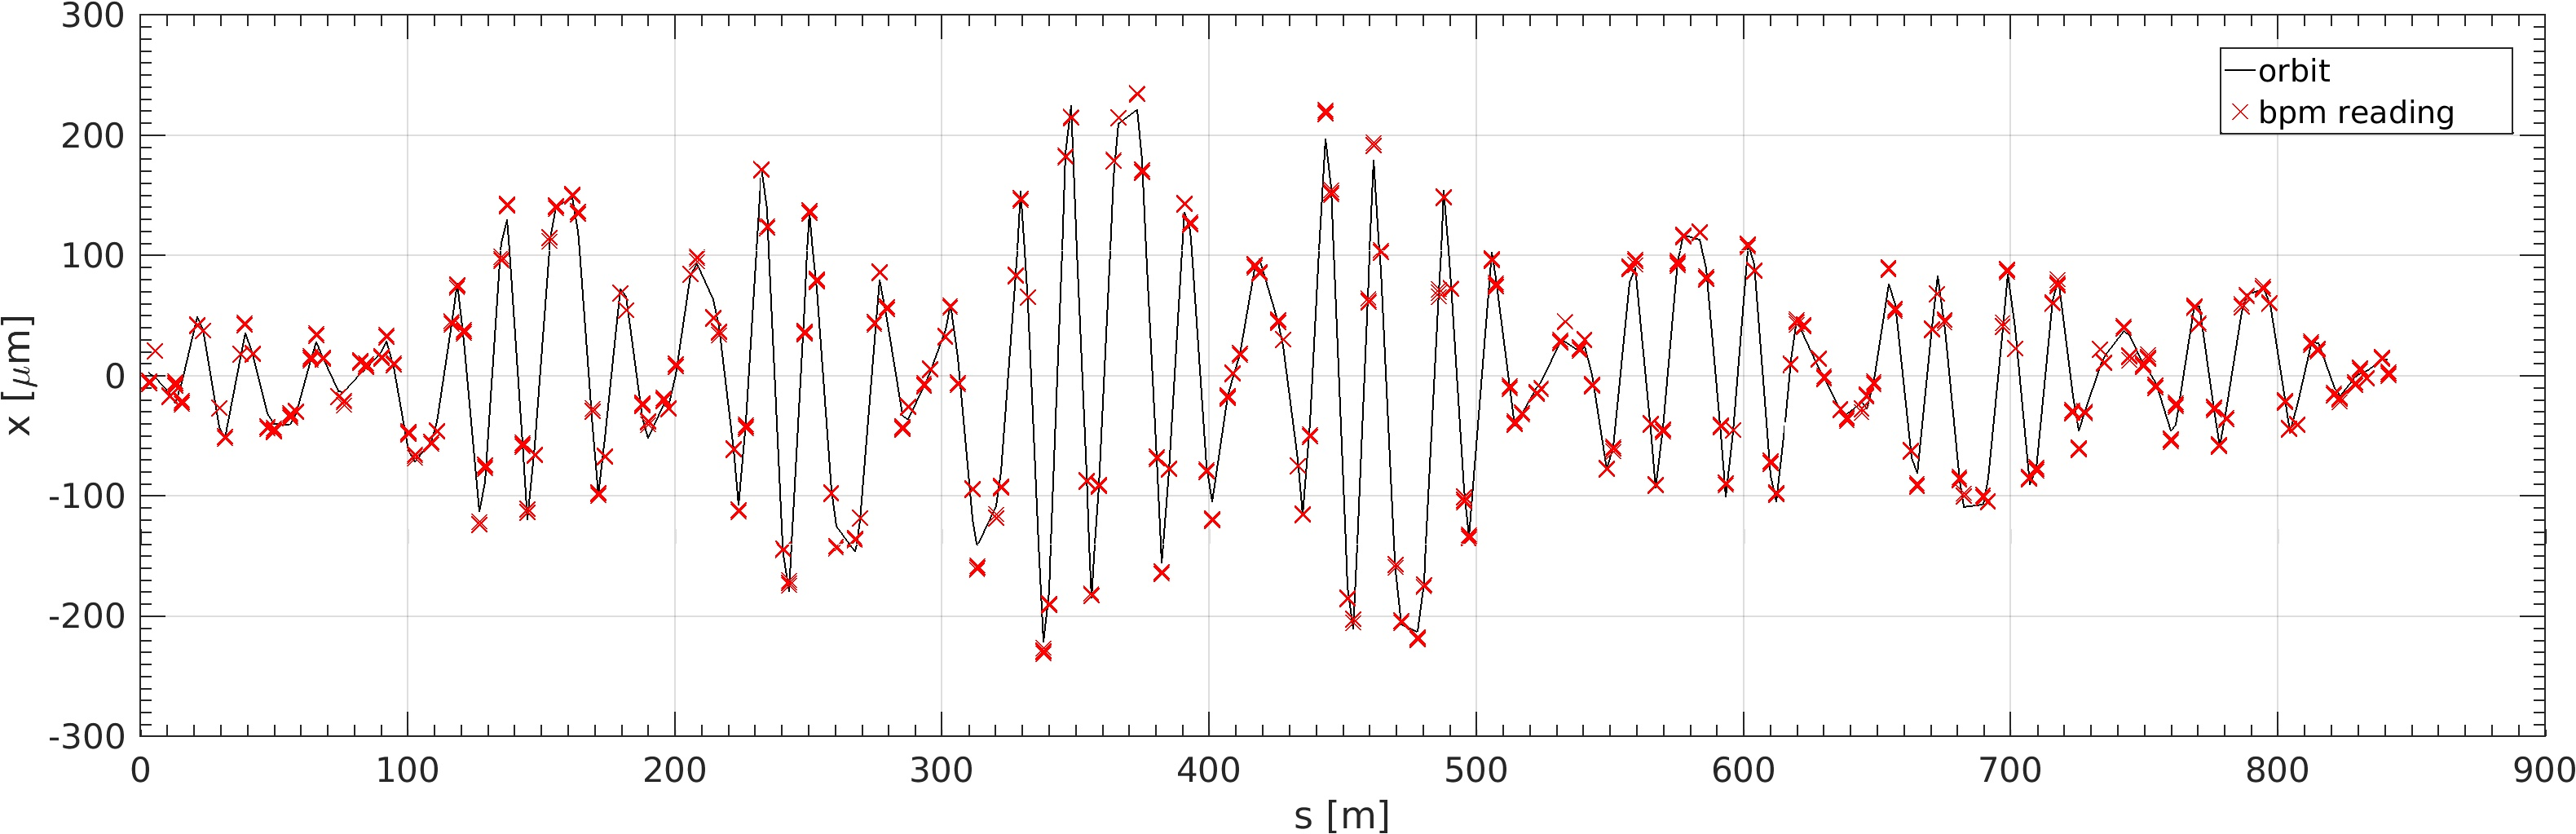
\includegraphics[width=0.98\textwidth]{./images/BPM/OrbitBPMAllErrX.jpg}
	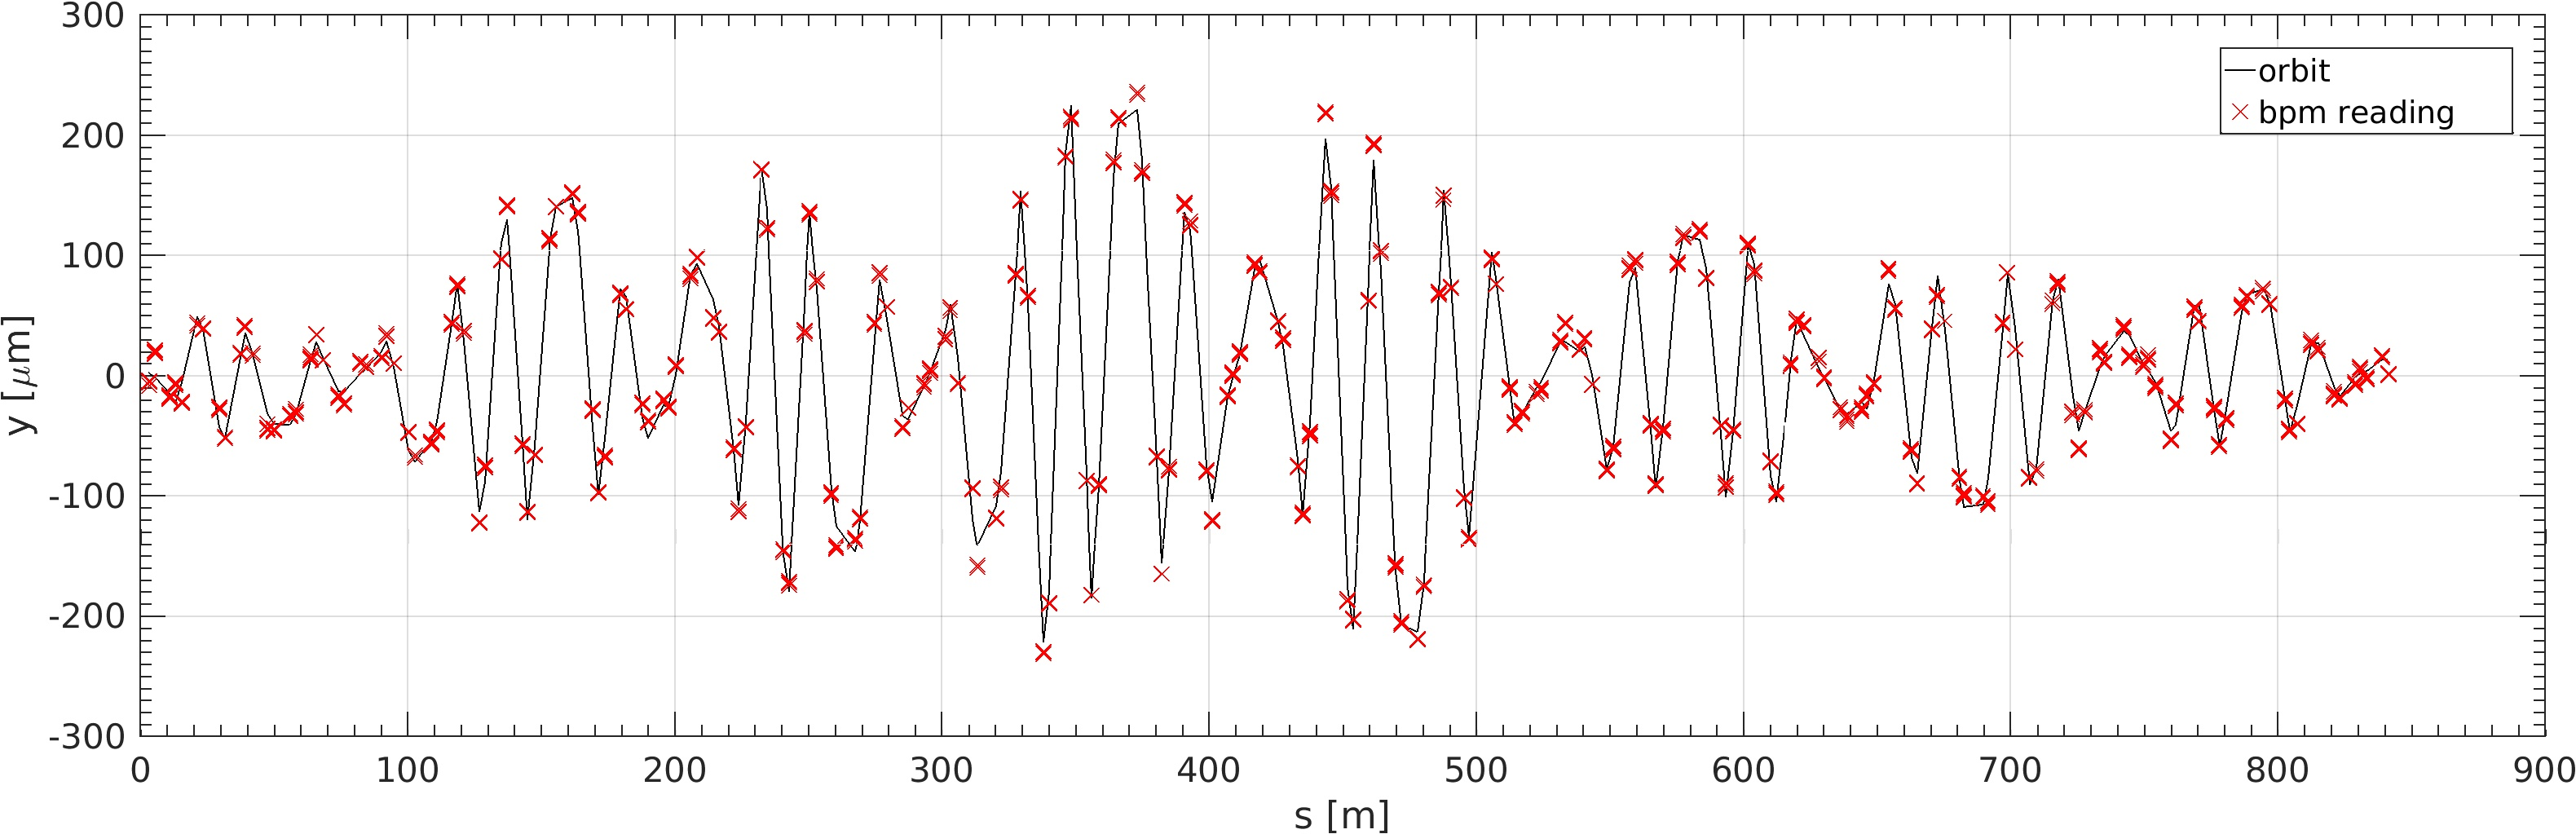
\includegraphics[width=0.98\textwidth]{./images/BPM/OrbitBPMAllErrY.jpg}
	\caption{Simulated orbit and 5 BPM orbit reading}
        \label{fig:diptiltref}
    \end{subfigure}
	\begin{subfigure}[b]{\textwidth}
   	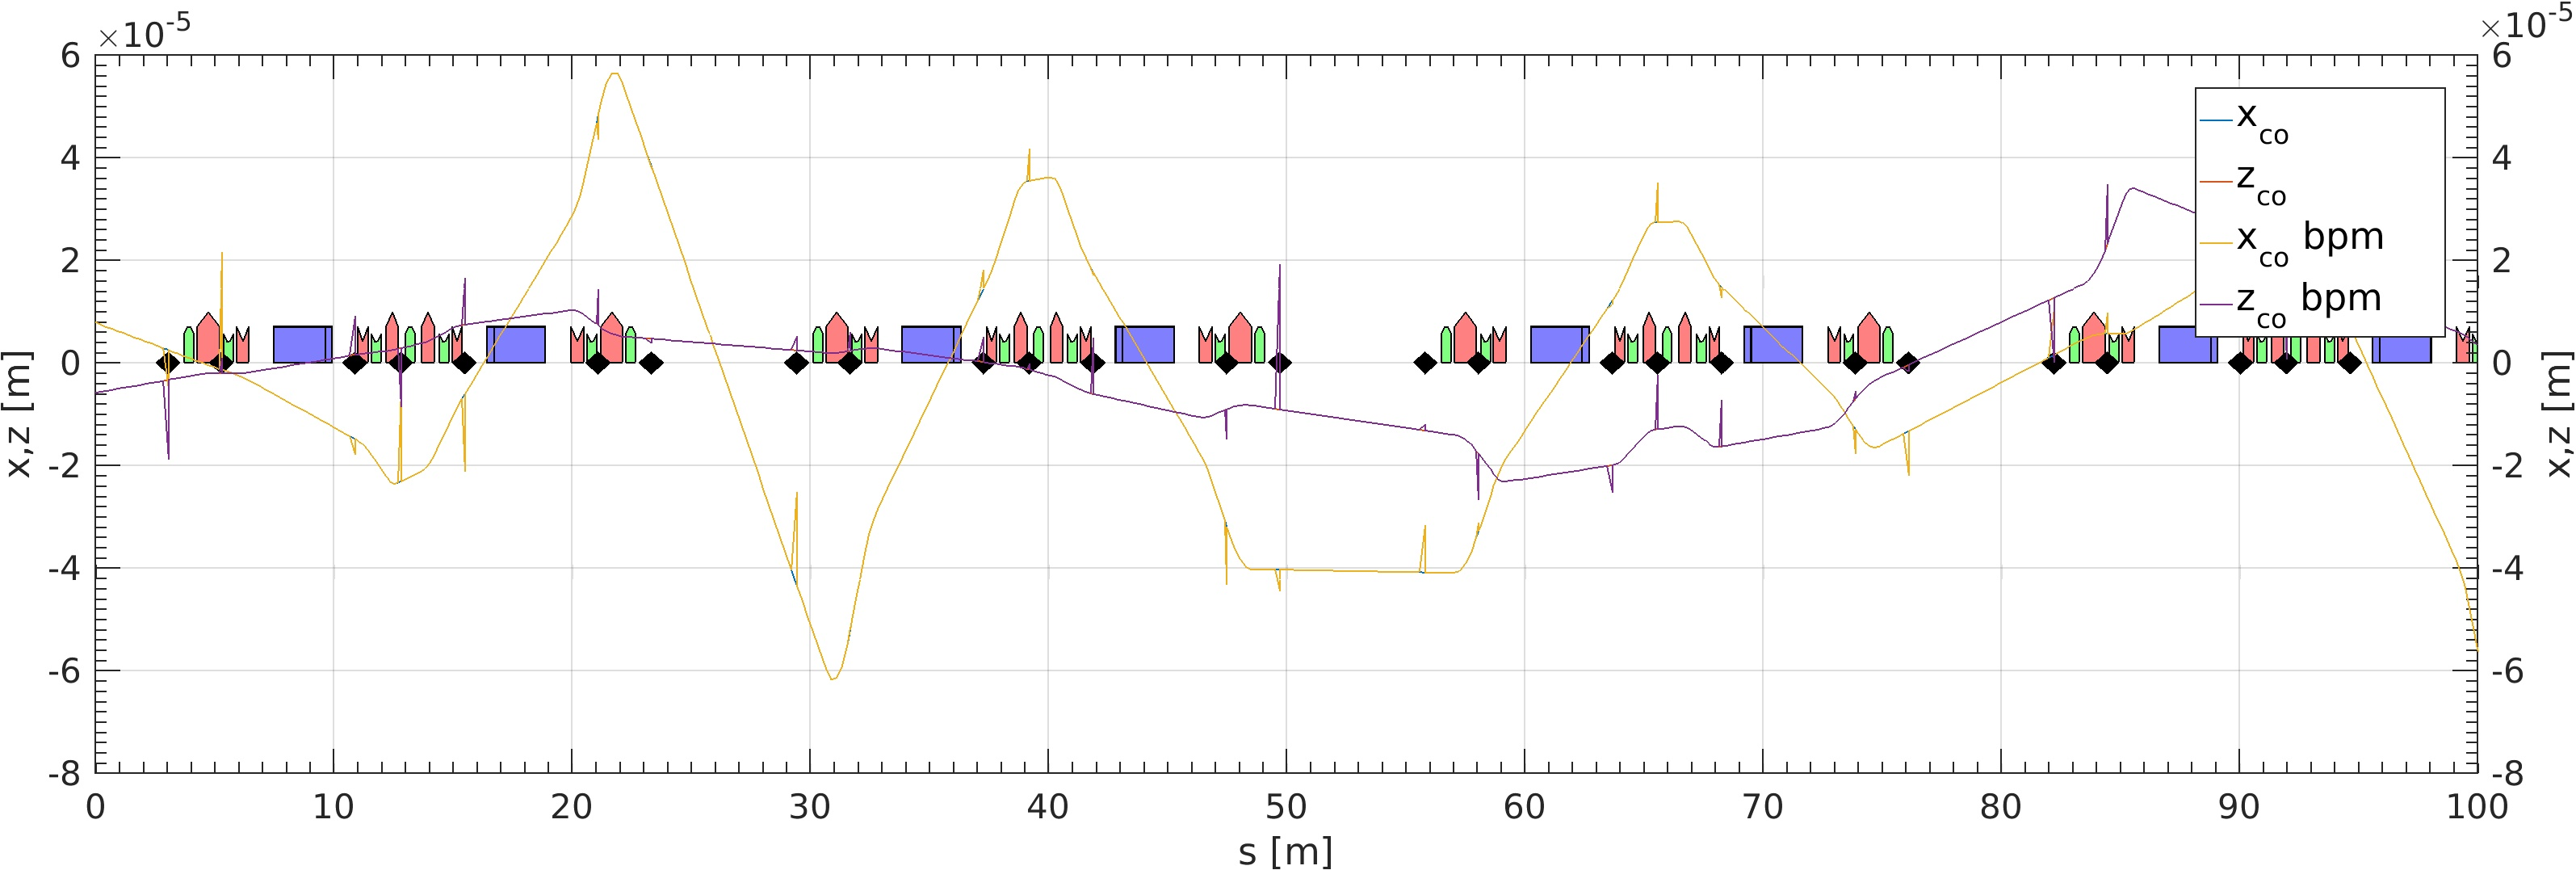
\includegraphics[width=0.98\textwidth]{./images/BPM/OrbitBPMAllErratplot.jpg}
	\caption{Difference between orbit and orbit reading displaied by \emph{atplot}}
        \label{fig:diptiltref}
    \end{subfigure}
	\caption{Orbit and BPM orbit reading.}
	\label{fig:bpmerr}
\end{figure}

\subsection*{functions used above}

\begin{itemize}
	\item atsetbpmerr
	\item findorbit4Err
	\item findorbit6Err
\end{itemize}

\clearpage
\subsection{Several errors in the lattice}
In most cases several errors need to be set in the lattice simultaneously. The function \emph{atsetrandomerrors} accepts a more structured input to simplify the specification of long lists of errors. A common seed is specified in order to have deterministic error sets. Below a sample of code and output errors, where several errors are specified and set simultaneously. The functions also considers splitted elements grouped using the \emph{MagGroup} flag in the AT structure fields. 

\begin{lstlisting}
% sextupoles
inds=findcells(r0,'Class','Sextupole');
errstruct(1).indx=inds;
errstruct(1).type='psi'; % roll
errstruct(1).sigma=200*1e-6;

% quadrupoles
indqm=[findcells(r0,'Class','Quadrupole')];
errstruct(2).indx=indqm;
errstruct(2).type='x';
errstruct(2).sigma=150*1e-6;
errstruct(3).indx=indqm;
errstruct(3).type='y';
errstruct(3).sigma=170*1e-6;

% girders
indg=[findcells(r0,'FamName','GS')];
errstruct(4).indx=indg;
errstruct(4).type='gx.gy';
errstruct(4).sigma=500*1e-6;

% set errors
magindex=arrayfun(@(a)a.indx,errstruct,'un',0);
type=arrayfun(@(a)a.type,errstruct,'un',0);
sigma=arrayfun(@(a)a.sigma,errstruct,'un',0);

rerr=atsetrandomerrors(...
    r0,...
    magindex,...  % cell array of indexes
    findcells(r0,'Class','Monitor'),...
    123456,...  % common seed
    sigma,...   % cell array of sigmas
    2.5,...     % truncation
    type);      % cell array of type
\end{lstlisting}

\begin{figure}[!h]
	\centering
	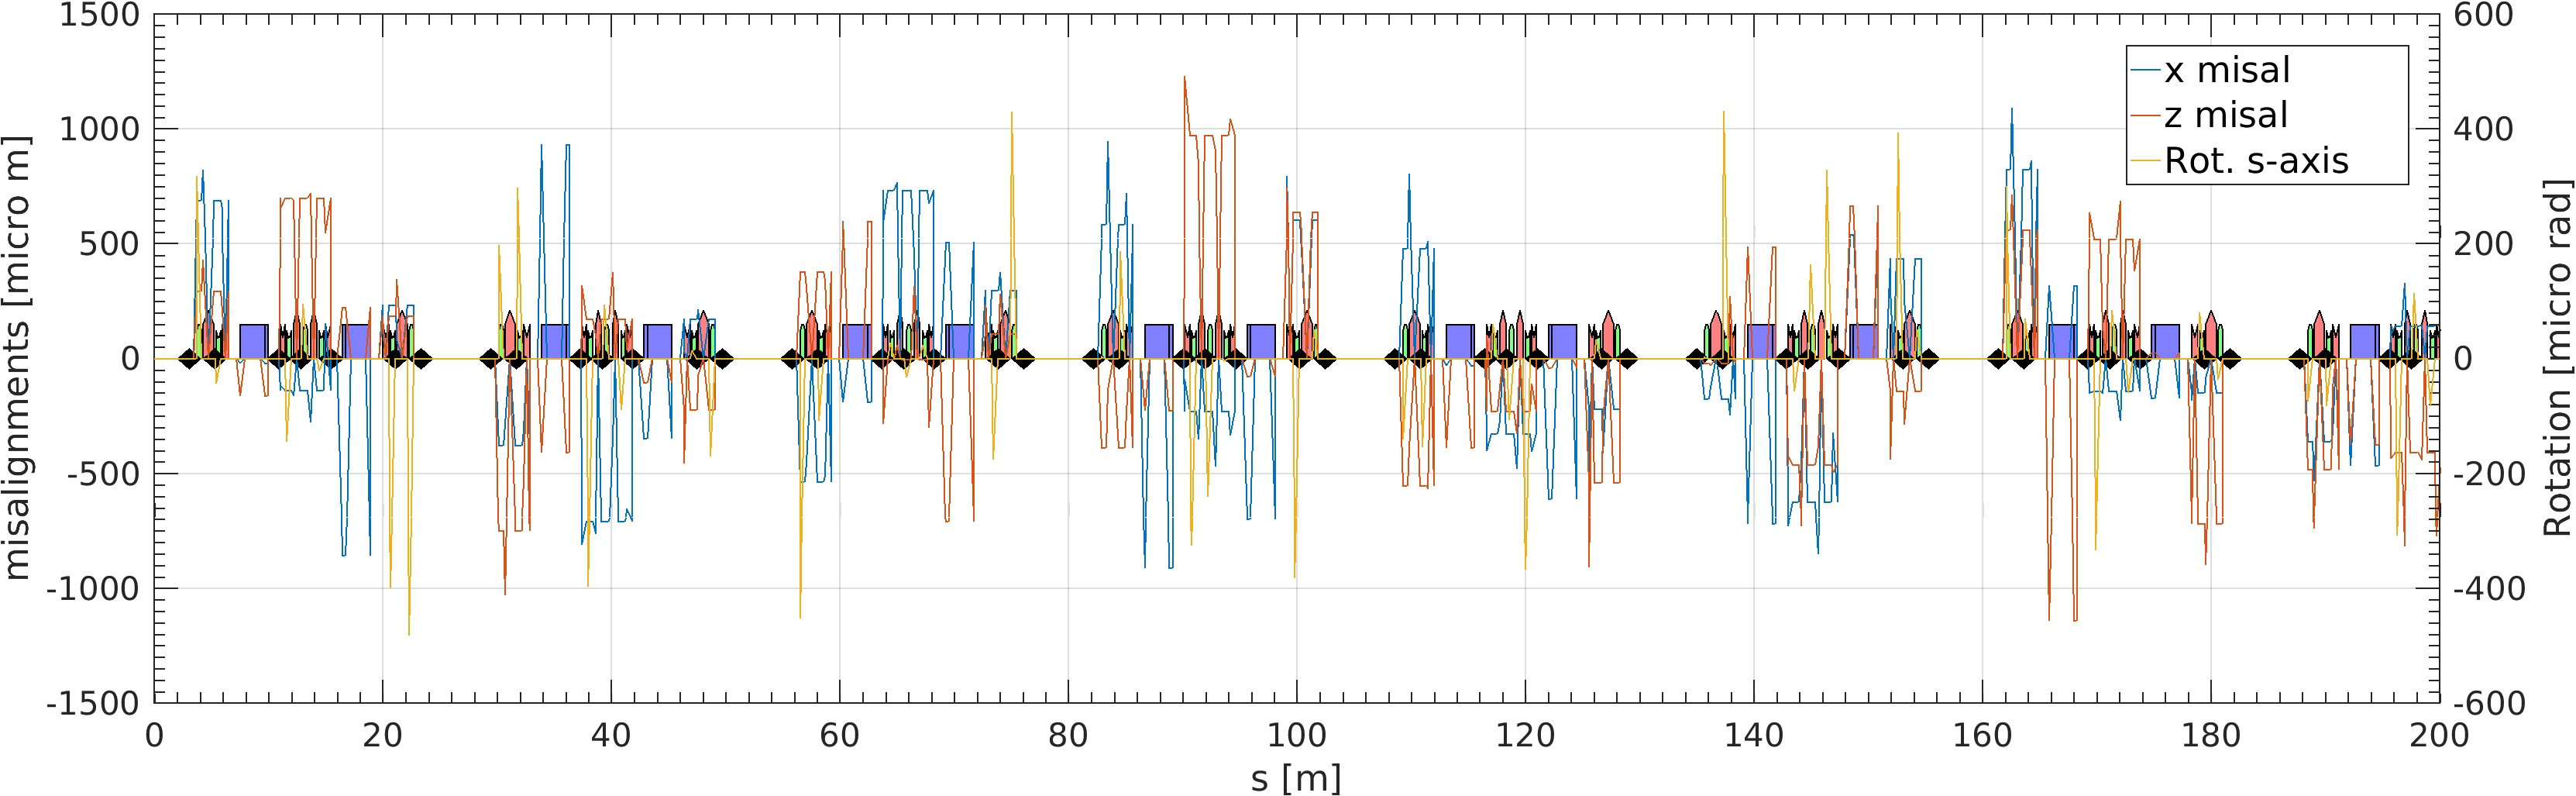
\includegraphics[width=0.98\textwidth]{./images/LargeList/LargeList.jpg}
	\caption{List of errors for different elements set using \emph{atsetrandomerrors}}
	\label{fig:girdxyrol}
\end{figure}
The errors that can be set are coded as follow:
\begin{itemize}
\item individual magnets: x, y, s, psi (roll), theta (yaw), phi (pitch), x.y, x.y.psi, x.y.s.psi, x.y.s.psi.theta.phi
\item bpm : bpm.offset, bpm.scale, bpm.read 
\item girders: gx, gy, gpsi, gtheta, gphi,  gx.gy, gx.gy.gpsi, gx.gy.gpsi.x.y.psi
\item main field components: dpb1, dpb2, dpb3, dpb4  
\end{itemize}

\clearpage
\subsection{Girder errors}
Girder errors can be implemented in two ways: moving by the same amount all elements that belong to a girder or setting the T1 and R1 field for the first elements and T2 and R2 field for the last one. 
The markers GS and GE define the start and end of Girders in the lattice and are used to specify the errors.
The first case is implemented in the function \emph{atsetrandomerrors} with error types \textit{gx, gy, gpsi, gx.gy} ...

\begin{lstlisting}
% get indexes
indm=find(atgetcells(ring,'Class','Monitor'));
% girders are defined by GS and GE markers (start and end of girder)
indg=find(atgetcells(ring,'FamName','GS')); 

% example: set pitch errors 
rerr=atsetrandomerrors(...
    ring,... % lattice
    indg,... % indexes
    indm,... % bpm indexes
    1,...    % seed
    1e-5,... % sigma or random error
    2.5,...  % number of sigmas for truncation
    'gphi'); % error kind
		
rerr2=atsetrandomerrors(...
    ring,... % lattice
    indg,... % indexes
    indm,... % bpm indexes
    1,...    % seed
    1e-5,... % sigma or random error
    2.5,...  % number of sigmas for truncation
    'gx.gy.gpsi'); % error kind

\end{lstlisting}


\begin{figure}[!h]
	\centering
	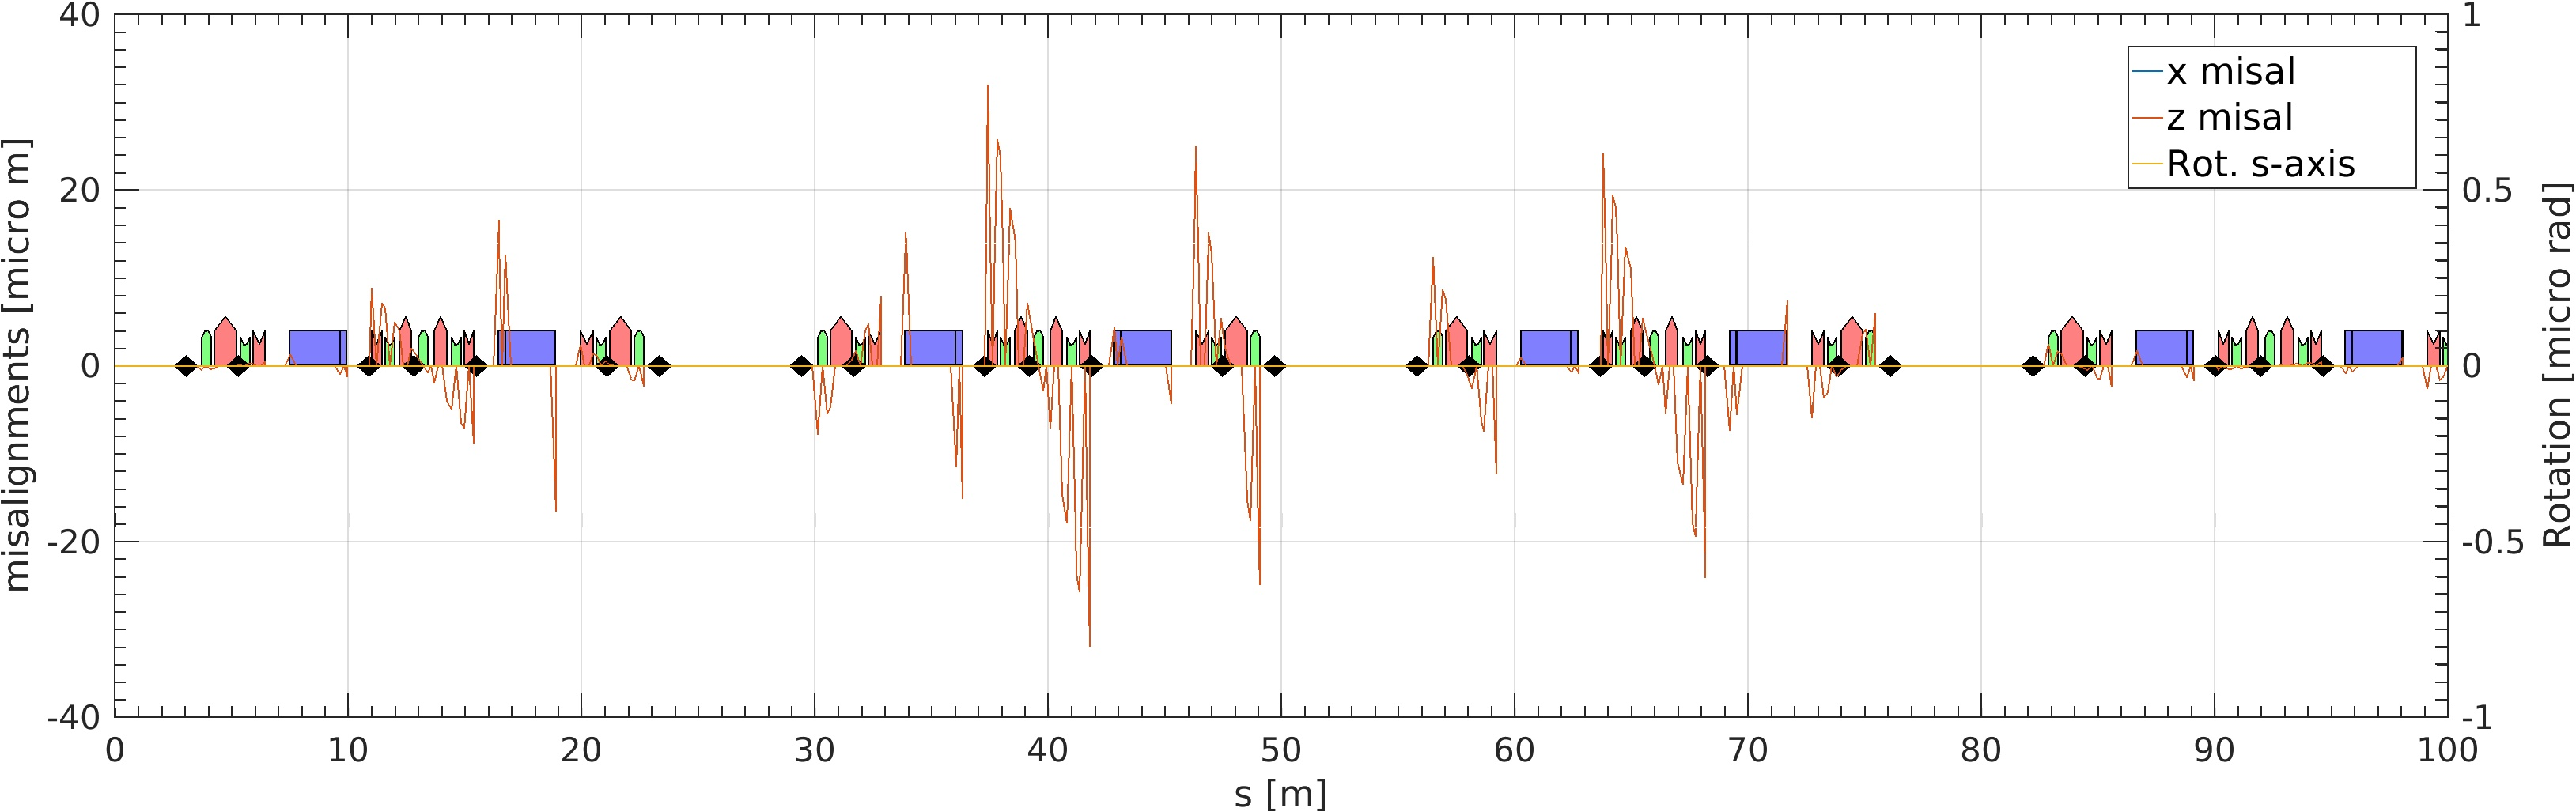
\includegraphics[width=0.98\textwidth]{./images/GIRDERS/GirderErrorsPitch.jpg}
	\caption{Girders pitch errors set using \emph{atsetrandomerrors}}
	\label{fig:girdpitch}
\end{figure}

\begin{figure}[!h]
	\centering
	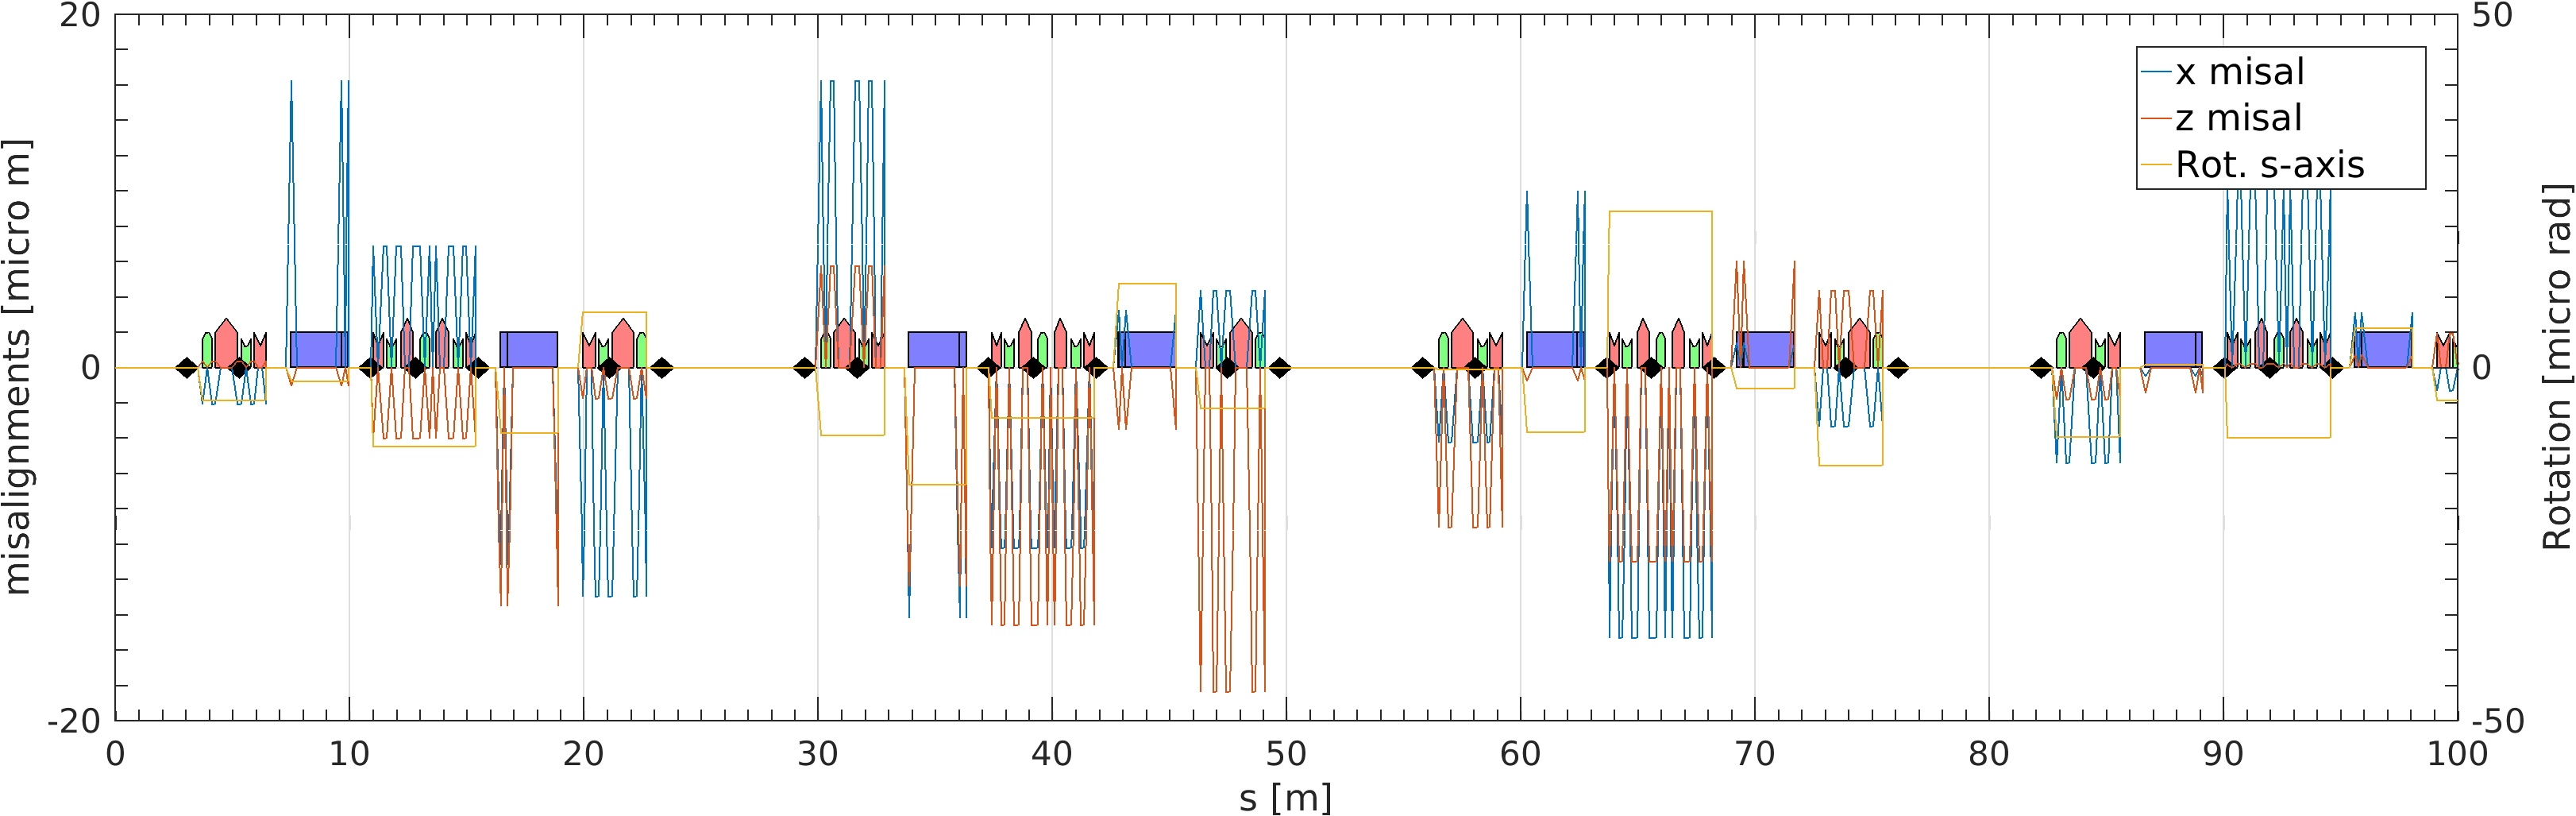
\includegraphics[width=0.98\textwidth]{./images/GIRDERS/GirderErrorsXYRoll.jpg}
	\caption{Girders horizontal, vertical and rotation about s errors set using \emph{atsetrandomerrors}}
	\label{fig:girdxyrol}
\end{figure}

\clearpage
\subsection{Survey errors}
Measurements of the positions of the accelerators are frequently performed. Knowing these measurement and their errors, it is also possible to simulate survey curves. This curves are a better estimation of the global alignment errors, and can eventually replace the girder-to-girder errors. If no measurements are available, studies of errors as shown in Sec. \ref{sec:ErrFreqDomain} can be performed. 

These errors can be very large, but as they are smoothly varying along the lattice, their effect is limited. BPM alignment errors (T1,R1,...) are used in \emph{findorbit4Err} and \emph{findorbit6Err} to offset the BPM reading. This defines a reference closed orbit that follows the global Survey curves. 


\begin{figure}[!h]
	\centering
	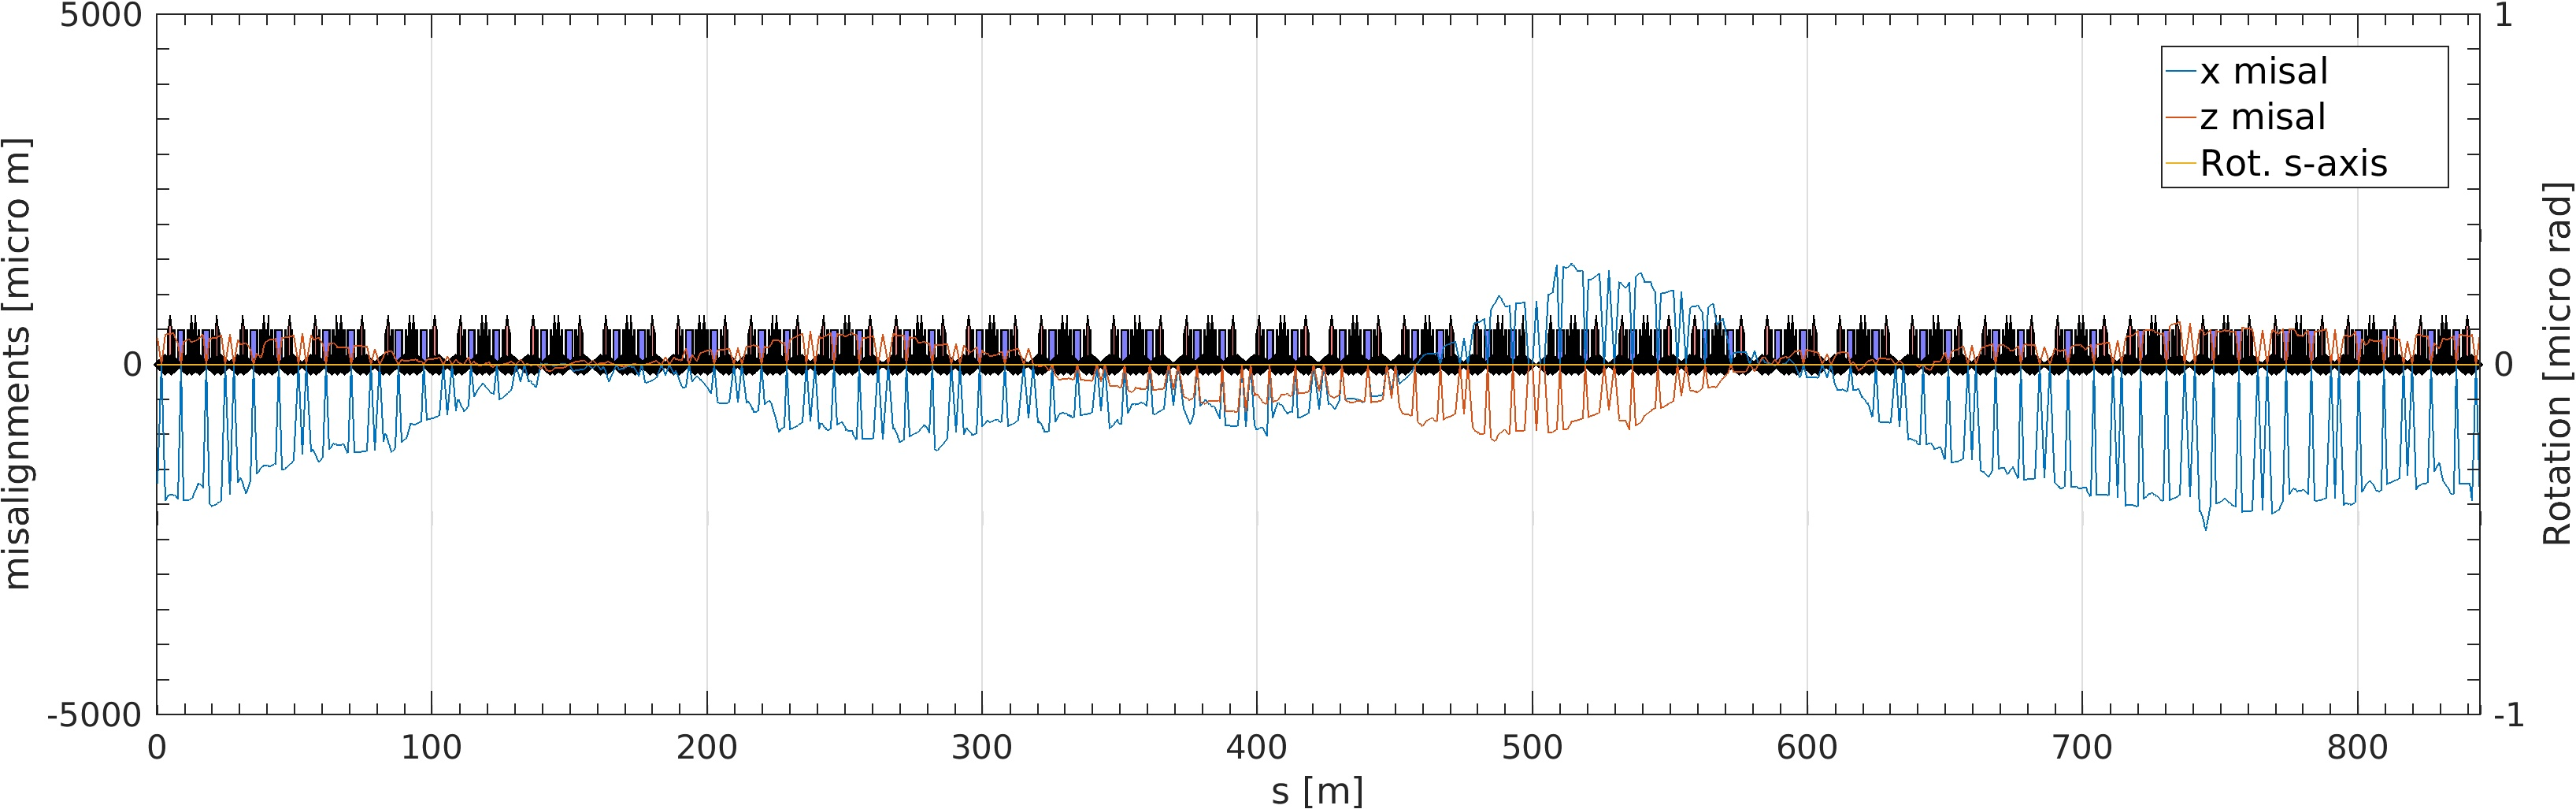
\includegraphics[width=0.98\textwidth]{./images/Survey/SurveyErrors.jpg}
	\caption{Survey Errors}
	\label{fig:girdxyrol}
\end{figure}


\subsection{Errors in frequency domain}
\label{sec:ErrFreqDomain}
Errors can be also studied in terms of frequency and amplitude. The function \emph{atsetwaveerrors} allows this kind of study. Below a sample of code and the resulting errors.

\begin{lstlisting}
ie=1;

wltouse=1:0.5:3;
amplx=0.6e-3;
amplY=0.6e-3;
amplpsi=0.6e-3;

W=findspos(r0,length(r0)+1)./wltouse;

A=amplx/length(W)*randn(size(W));
errwavestruct(ie).indx=1:length(r0);%findcells(r0,'Class','Quadrupole');
errwavestruct(ie).type='x';
errwavestruct(ie).A=A(end:-1:1);
errwavestruct(ie).W=W;
ie=ie+1;

A=amplY/length(W)*randn(size(W));
errwavestruct(ie).indx=1:length(r0);%findcells(r0,'Class','Quadrupole');
errwavestruct(ie).type='y';
errwavestruct(ie).A=A(end:-1:1);
errwavestruct(ie).W=W;
ie=ie+1;

A=amplpsi/length(W)*randn(size(W));
errwavestruct(ie).indx=1:length(r0);%findcells(r0,'Class','Quadrupole');
errwavestruct(ie).type='psi';
errwavestruct(ie).A=A(end:-1:1);
errwavestruct(ie).W=W;
ie=ie+1;

magindex=arrayfun(@(a)a.indx,errwavestruct,'un',0);
type=arrayfun(@(a)a.type,errwavestruct,'un',0);
A=arrayfun(@(a)a.A,errwavestruct,'un',0);
W=arrayfun(@(a)a.W,errwavestruct,'un',0);

rerr=atsetwaveerrors(...
    r0,...
    magindex,...
    findcells(r0,'Class','Monitor'),...
    W,...
    A,...
    type);

\end{lstlisting}

\begin{figure}[!h]
	\centering
	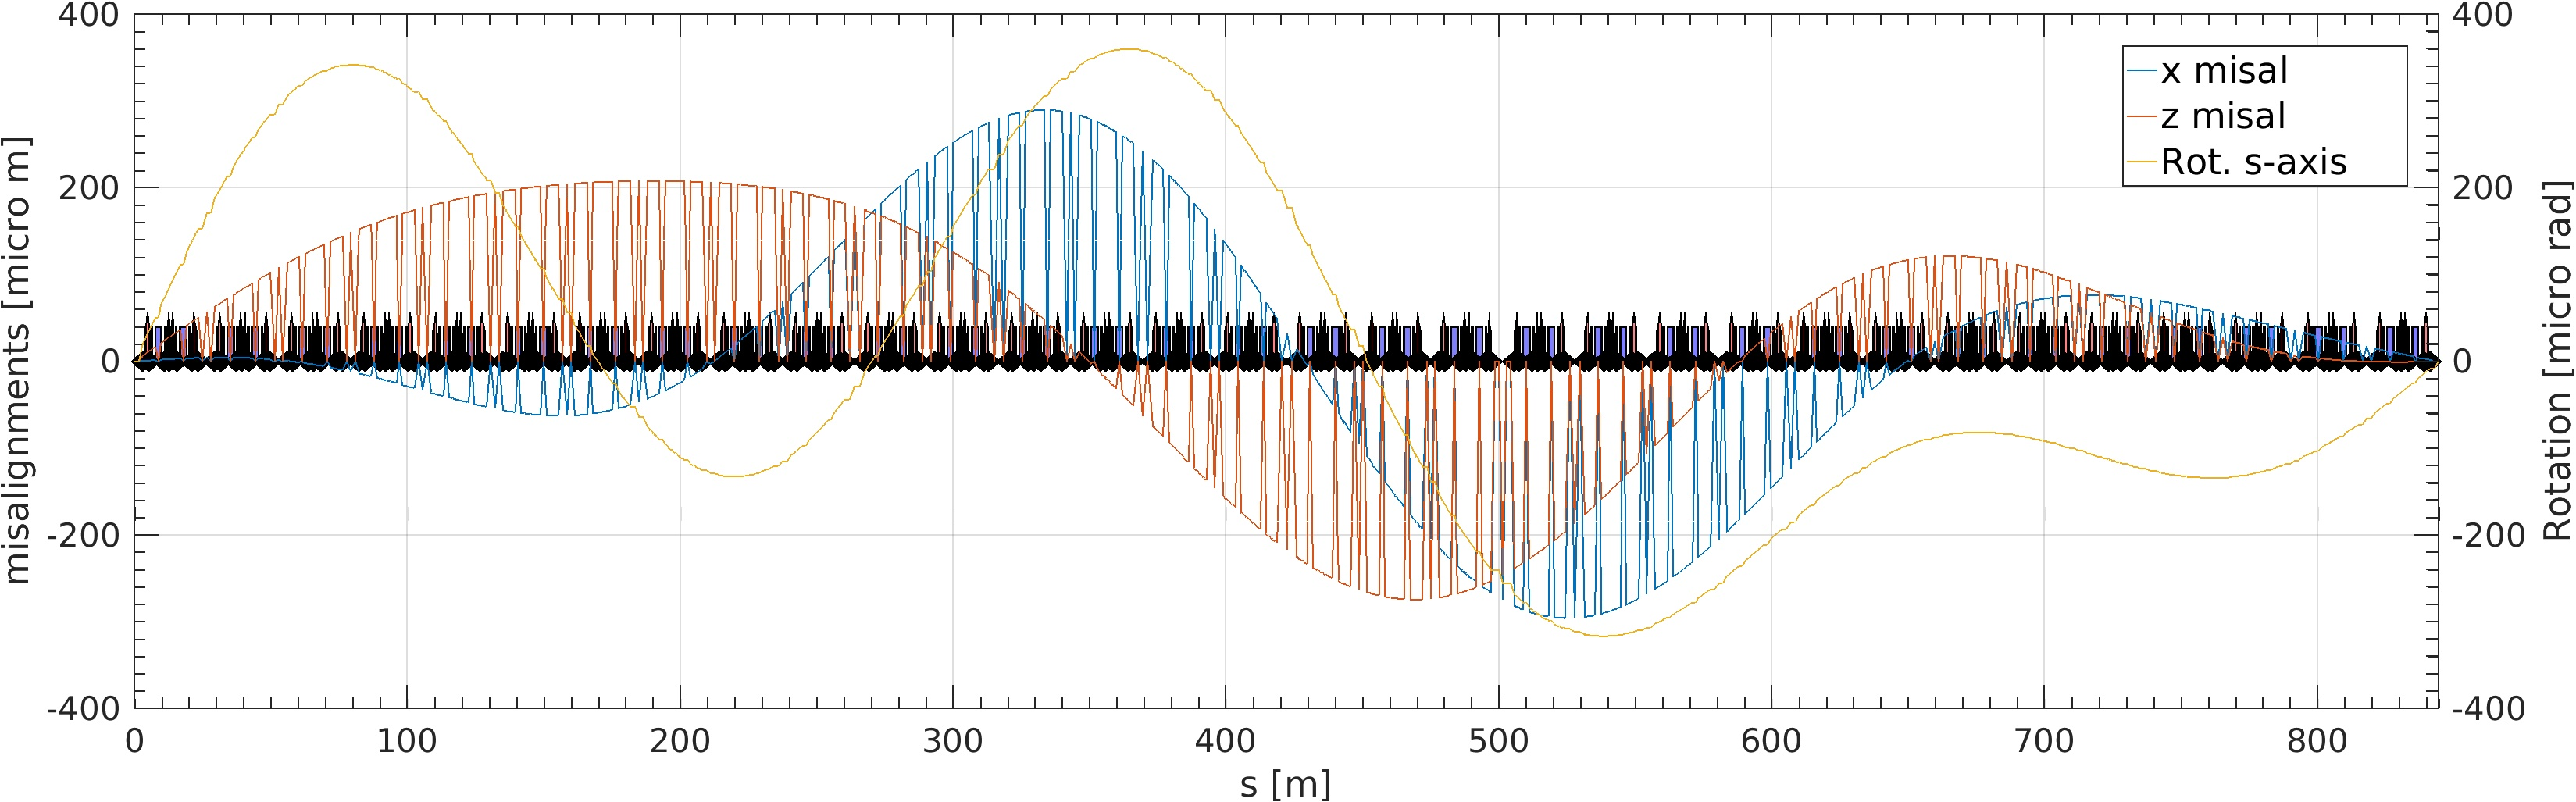
\includegraphics[width=0.98\textwidth]{./images/Wave/Wave.jpg}
	\caption{List of low frequency errors (sum of several frequency and amplitudes) for different errors set using \emph{atsetwaveerrors}}
	\label{fig:girdxyrol}
\end{figure}


\clearpage
\subsection{Main field errors}
To set main field errors the options of \emph{atsetrandomerrors}, \textit{dpb1, dpb2, dpb3, dpb4} can be used.
\begin{lstlisting}
% get indexes
indm=find(atgetcells(ring,'Class','Monitor'));
indq=find(atgetcells(ring,'Class','Quadrupole')); % girders are defined by GS and GE markers (start and end of girder)

rerr=atsetrandomerrors(...
    ring,... % lattice
    indq,... % quad indexes
    indm,... % bpms
    1,...    % seed
    1e-1,... % errors of 10%
    2.5,...  % truncation
    'dpb2'); % error type: dpb1, dpb2, dpb3, dpb4
		
\end{lstlisting}


\begin{figure}[!h]
	\centering
	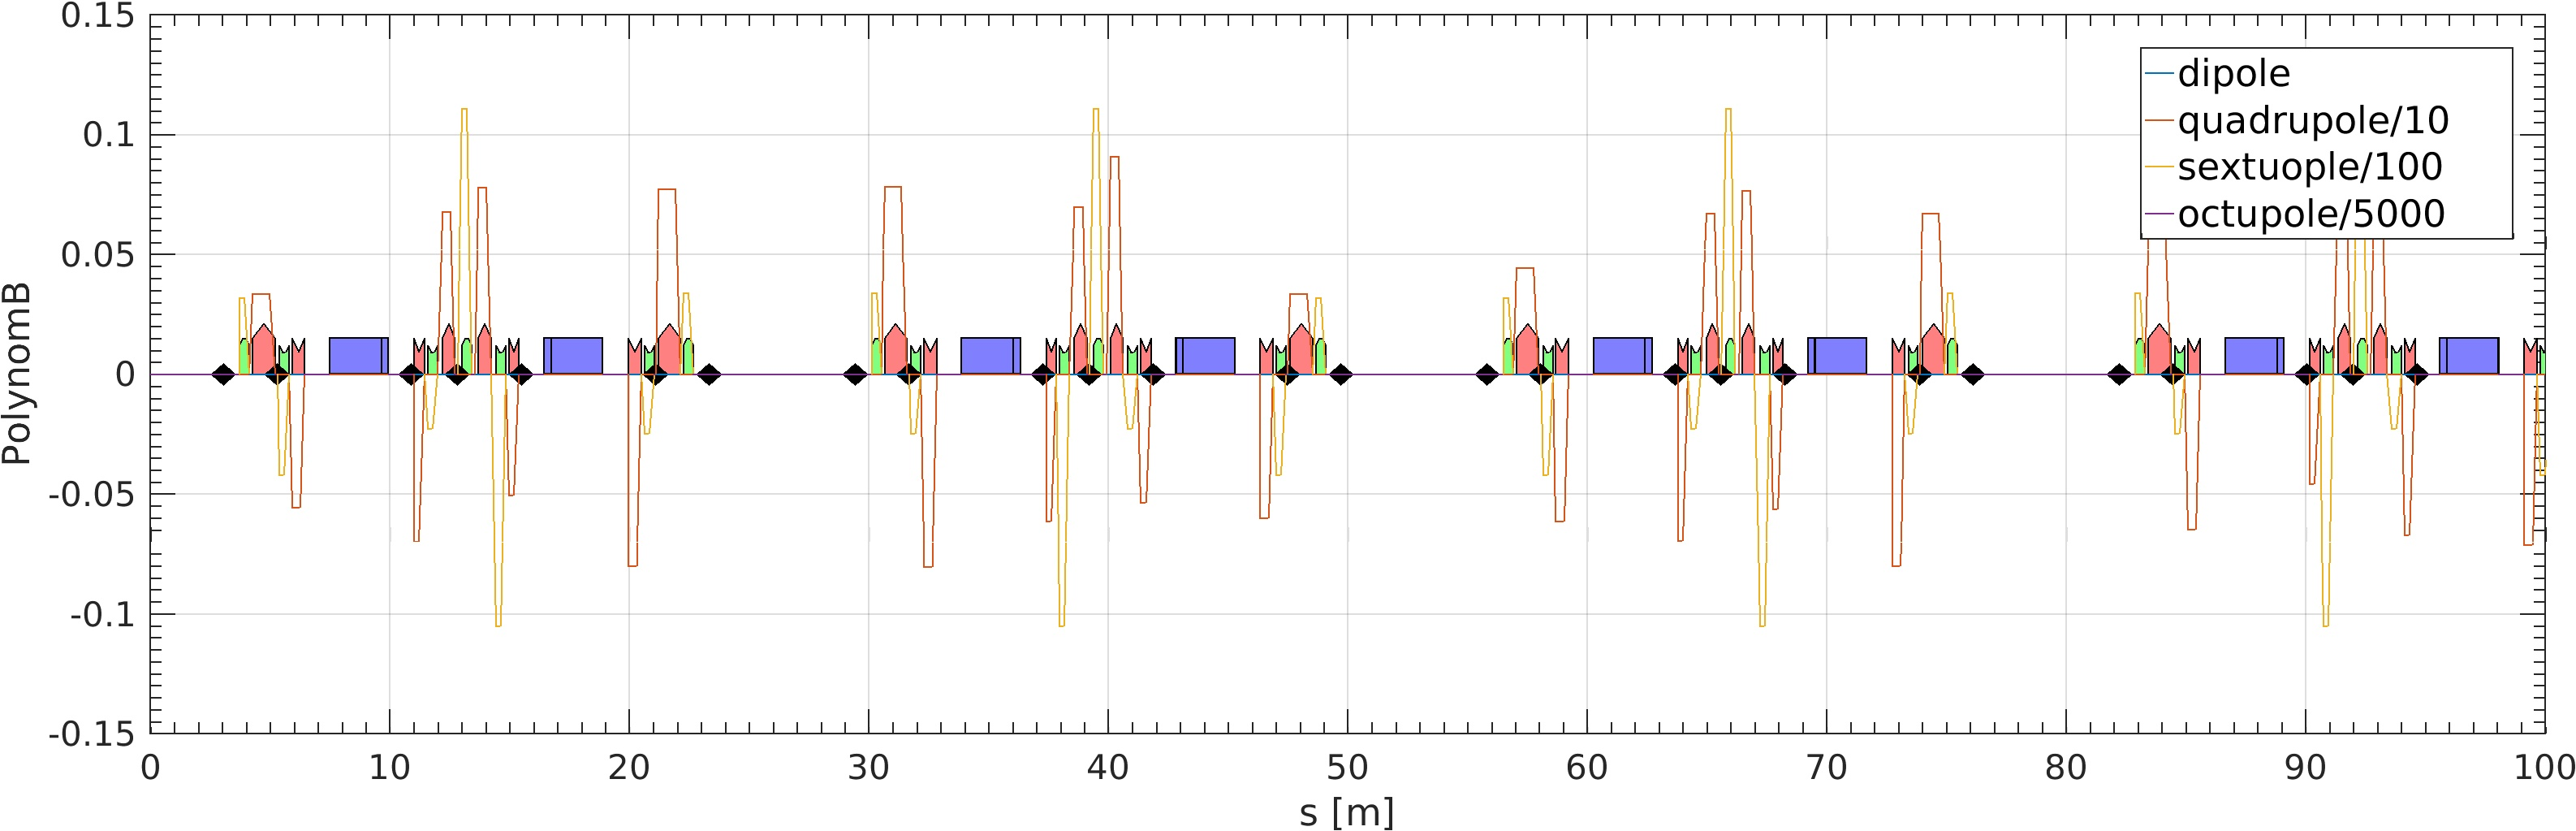
\includegraphics[width=0.98\textwidth]{./images/FieldIntegral/FieldIntegral.jpg}
	\caption{Quadrupole field errors set using \emph{atsetrandomerrors}}
	\label{fig:girdpitch}
\end{figure}

\clearpage
\subsection{Multipole errors}
Multipole errors may be systematic or random. To set on a given magnet a series of multipole errors, in AT is sufficient to state them in PolynomB and PolynomA, and increase accordingly the MaxOrder field of the element.
However care has to be taken since different conventions might be used for the magnetic field decomposition. The field decomposition in AT is: 
$$
B=B\rho*\Sigma_{n=1}^{\infty}((b_n+i*a_n)(z)^(n-1)) 
$$
where $b_n$ and $a_n$ are PolynomB and PolynomA while for the magnet design group of ESRF is:
$$
B=B_N(\rho_0)*\Sigma_{n=1}^{\infty}((B_{N,n}+i*A_{N,n})(\frac{z}{\rho_0})^{n-1})
$$
where $\rho_0$ is the reference radius and $B_{N,n}$, $A_{N,n}$ the multipole components.

The function \emph{AssignFieldErr} does the conversion and sets the multipole errors, scaling with the main field. 

\begin{lstlisting}
% get indexes
indq=find(atgetcells(ring,'Class','Quadrupole'));

% set multipole errors
bn=[0 0 0 0 0 1.10934 0 0 0 -5.18658]*1e-4;

an=[
    0
    0
    4.803458371
    1.910276957
    1.055734675
    0.588073151
    0.312742308
    0.175288289
    0.101114708
    0.064747269]'*1e-4;

[rerr,PolB,PolA]=AssignFieldErr(ring,indq,2,7*1e-3,bn,an);

\end{lstlisting}

\clearpage
\subsubsection*{Multipole errors in correctors}
In the case of correctors magnets, the multipole errors must be updated every time the correctors change strength. 

\clearpage
\subsection{Retrieving and displaying the errors values in AT}
